% This example is meant to be compiled with lualatex or xelatex
% The theme itself also supports pdflatex
\PassOptionsToPackage{unicode}{hyperref}
\documentclass[aspectratio=1610, xcolor=dvipsnames, 9pt]{beamer}

% Load packages you need here
\usepackage{polyglossia}
\setmainlanguage{german}

\usepackage{csquotes}
\usepackage{smartdiagram}

\usepackage{amsmath}
\usepackage{amssymb}
\usepackage{mathtools}

\usepackage{hyperref}
\usepackage{bookmark}

% load the theme after all packages

\usetheme[
  showtotalframes, % show total number of frames in the footline
]{fhswf}

% Put settings here, like
\unimathsetup{
  math-style=ISO,
  bold-style=ISO,
  nabla=upright,
  partial=upright,
  mathrm=sym,
}

\title{Neuronale Netze/Deep Learning und Predictive Maintenance}
\author[F.~Neubürger, T.~Kopinski]{ \textbf{Felix Neubürger}, Prof. Dr. Thomas Kopinski}
\institute[I \& W]{Fachhochschule Südwestfalen, Ingenieurs- \& Wirtschaftswissenschaften}
\date{15. Juni 2024}
\titlegraphic{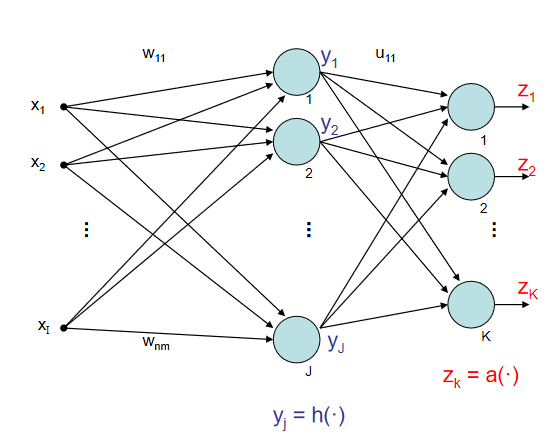
\includegraphics[width=0.2\textwidth]{images/MLP2.png}}


\begin{document}

\maketitle
\begin{frame}{Abfrage Erwartungen und Vorwissen}
  \begin{columns}
    \begin{column}{1\textwidth}
      \begin{itemize}
        \item \url{https://www.menti.com/} \newline
        \item Code: 3972 7236
      \end{itemize}
    \end{column}
    \begin{column}{0\textwidth}
% \begin{figure}
% \centering
%             \includegraphics[width=0.9\textwidth]{images/intro/intro.pdf}
% \end{figure}
    \end{column}
  \end{columns}
\end{frame}

\begin{frame}{Inhalte der Vorlesung}
  \begin{columns}
    \begin{column}{1\textwidth}
      \begin{itemize}
        \item Wiederholung Neuronale Netze (NN)\newline
        \item Einführung spezieller Architekturen Neuronaler Netze \newline
        \item Anwendung von Neuronalen Netzen zur Lösung zur Datenanalyse  \newline
        \item Verschiedene Architekturen Neuronaler Netze \newline 
        \item Einführung in das Anwendungsthema der Predictive Maintenance (PM) \newline
        \item Bearbeitung von Benchmark Datensätzen in der PM mithilfe von NN \newline
        \item Strategien zur Durchführung von PM Projekten
      \end{itemize}
    \end{column}
    \begin{column}{0\textwidth}
% \begin{figure}
% \centering
%             \includegraphics[width=0.9\textwidth]{images/intro/intro.pdf}
% \end{figure}
    \end{column}
  \end{columns}
\end{frame}

\begin{frame}{Ziele der Vorlesung - Welche Fragen sollen beantwortet werden?}
  \begin{columns}
    \begin{column}{0.69\textwidth}
      \begin{itemize}
        \item Was genau machen Neuronale Netze? \newline
        \item Wie kann ich mir das vorstellen? \newline
        \item Was ist überhaupt "Deep Learning"?  \newline
        %\item Welche Vorteile kann Predictive Maintenance haben? \newline
        \item Welche verschiedenen Architekturen neuronaler Netze gibt es? \newline
        \item Muss es immer Deep Learning sein? \newline
        %\item Wie gehe ich an ein Predictive Maintenance Projekt heran?
      \end{itemize}
    \end{column}
    \begin{column}{0.3\textwidth}
 \begin{figure}
 \centering
             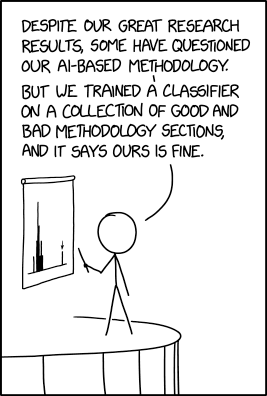
\includegraphics[width=0.9\textwidth]{images/ai_methodology.png}
             [\url{https://xkcd.com/2451/}]
 \end{figure}
    \end{column}
  \end{columns}
\end{frame}

\begin{frame}{Fromat der Vorlesung - Wie sollen diese Fragen beantwortet werden?}
  \begin{columns}
    \begin{column}{0.69\textwidth}
      \begin{itemize}
        \item Theroretischer Teil mit Folien \newline
        \item Praktischer Teil in Gruppen an einem Projekt  \newline
        \item Gruppengröße 2 oder 3 Personen  \newline
        %\item Welche Vorteile kann Predictive Maintenance haben? \newline
        \item Einzelarbeit möglich wenn eigenes Thema vorhanden \newline
        \item Abgabe der Ausarbeitung eine Woche vor der Blockwoche \newline
        \item Vorstellung der Projektergebnisse in der Blockwoche \newline
        \item Gewichtung der Bewertung Projektausarbeitung (70\%) und Vortrag (30\%)
        %\item Wie gehe ich an ein Predictive Maintenance Projekt heran?
      \end{itemize}
    \end{column}
    \begin{column}{0.3\textwidth}
 \begin{figure}
 \centering
             
\includegraphics[width=0.7\textwidth]{images/tasks.png} \newline
             [\url{https://xkcd.com/1425/}]
 \end{figure}
    \end{column}
  \end{columns}
\end{frame}

\begin{frame}{Was ist Predictive Maintenance?}
  \begin{columns}
    \begin{column}{1\textwidth}
      Grundlegende Ziele
      \begin{itemize}
        \item Prozessüberwachung und eventuelle Steuerung \newline
        \item Vorhersagen von Maschinen/Produktionsausfällen \newline
        \item Hilfe/Unterstützung bei der Wartungsplanung \newline
        \item Klassifikation von Fehlerzuständen \newline
      \end{itemize}
    \end{column}
    % \begin{column}{0.4\textwidth}
    %   \begin{figure}
    %     \centering
    %      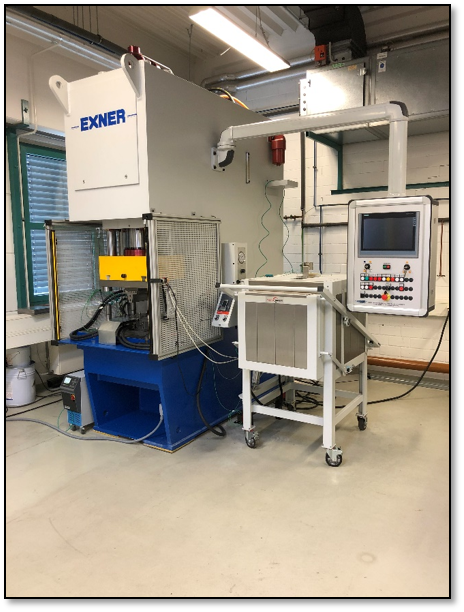
\includegraphics[width=0.6\textwidth]{images/anlage.png}
    %   \end{figure}
    % \end{column}
  \end{columns}
    \end{frame}


  \begin{frame}{Was sind Neuronale Netze und was ist Deep Learning?}
        \begin{columns}
          \begin{column}{0.7\textwidth}
            \begin{itemize}
              \item Abstrakt: Verkettung nichtlinearer Abbildungen \newline
              \item Die Parameter dieser Abbildungen wird mit vorhandenen Daten "gelernt" \newline
              \item Verschiedene Optimierungsverfahren zur Festlegung der "besten" Parameter \newline
            \end{itemize}
          \end{column}
          \begin{column}{0.3\textwidth}
       \begin{figure}
       \centering
                   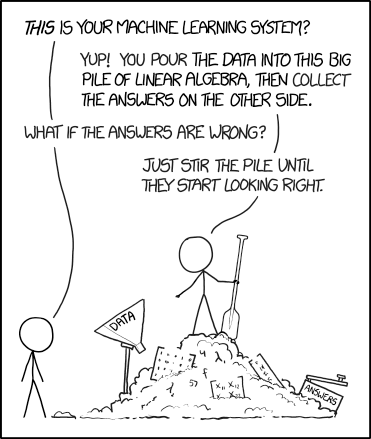
\includegraphics[width=0.9\textwidth]{images/machine_learning.png}\newline
             [\url{https://xkcd.com/1838/}]
       \end{figure}
          \end{column}
        \end{columns}
      \end{frame}
\begin{frame}{Konstruktion von Neuronalen Netzen: Single-Layer-Perceptron}
        \begin{columns}
          \begin{column}{0.7\textwidth}
            \begin{itemize}
              \item Einfacher binärer Klassifikator
              \begin{equation}
                        f(\text{x}) = \begin{cases}1 & \text{if }\ w \cdot x + b > \Theta,\\0 & \text{otherwise}\end{cases}
                    \end{equation}
              \item mit dem Gewichtsvektor $w$, dem Skalarprodukt $w\cdot x= \sum_{i=1}^{m} w_i x_i$ mit der Inputdimension $m$ und dem biasvektor $b$ \newline
              \item dieser klassifikator beschreibt im zwei dimensionalen Fall eine Halbebene im Koordinatensystem mit 
              \begin{align}
                w_1 x + w_2 y &> \Theta \\
                y &> - \frac{w_1}{w_2} x -\Theta
              \end{align}
              \item Anschaulich: Alle Punkte über dieser Linie werden der Klasse 1 zugeordnet und alle unterhalb dieser Linie der Klasse 0
            \end{itemize}
          \end{column}
          \begin{column}{0.3\textwidth}
       \begin{figure}
       \centering
                   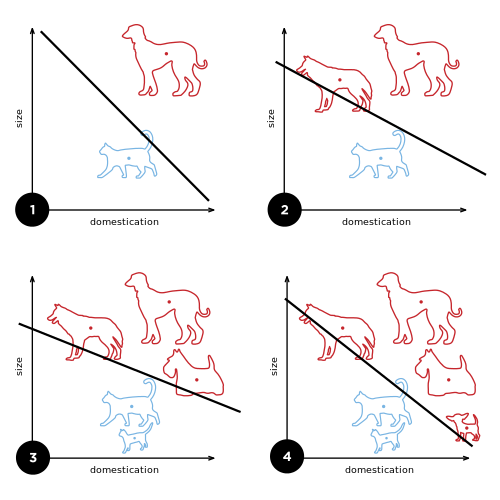
\includegraphics[width=0.9\textwidth]{images/Perceptron_example.svg.png}
       \end{figure}
          \end{column}
        \end{columns}
      \end{frame}

      \begin{frame}{Training von Neuronalen Netzen: Single-Layer-Perceptron}
        \begin{columns}
          \begin{column}{0.7\textwidth}
            \begin{itemize}
              \item Optimierung dieser gewicht für einen gegebenen Datensatz mit den Datenpunkten $x$ aus der Gesamtmenge $B$
              \item Update der Gewichte durch:
                    \begin{equation}
                       w ^{(t+1)} = w^t + \gamma \sum_{w'^t x <0, x \in B} x \text{ mit der learning rate:   } \gamma>0
                    \end{equation}
              \item mit der Menge der Fehlklassifizierungen im Schritt $t$: $F(w) = \{x \in B : w'x<0 \}$
              \item Daraus folgt die zu optimierende Zielfunktion: $ f(w) = -\sum_{F(w)} w'x $ \rightarrow min \newline
              \item Anschaulich: Wir optimieren die Gewichte so lange bis die Zielfunktion $f(w)=0$ ist, da dann $F(w)=\emptyset$ \newline

              \item Ist das immer erreichbar?
            \end{itemize}
          \end{column}
          \begin{column}{0.3\textwidth}
       \begin{figure}
       \centering
                   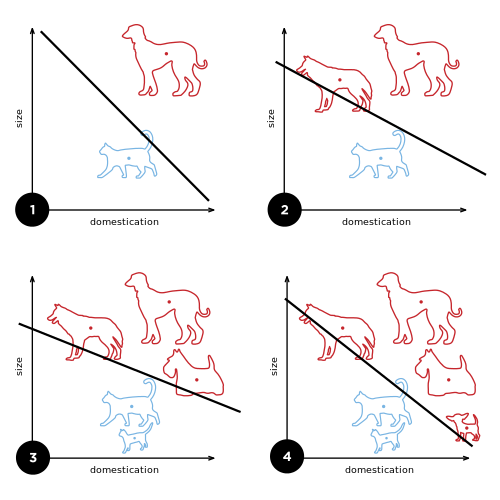
\includegraphics[width=0.9\textwidth]{images/Perceptron_example.svg.png}
       \end{figure}
          \end{column}
        \end{columns}
      \end{frame}

      \begin{frame}{Training von Neuronalen Netzen: Single-Layer-Perceptron}
        \begin{columns}
          \begin{column}{0.7\textwidth}
            \begin{itemize}
              \item Wie erreichen wir diese Bedingung?
              \item \emph{gradient descent}
                    \begin{equation}
                       w^{(t+1)} = w^t - \gamma \nabla f(w^t)  \text{ mit:   } \gamma>0
                    \end{equation}
              \item Exkurs Analysis: Der Gradient zeigt immer in die Richtung des steilsten Anstiegs einer Funktion
              \item Daraus folgt, dass die Nacheinanderausführung dieser Iteration in einem lokalen Minimum konvergiert 
              \item \begin{align}
                \nabla f(w) &= \left( \frac{\partial f(w)}{\partial w_1}, \frac{\partial f(w)}{\partial w_2}, ... ,\frac{\partial f(w)}{\partial w_n} \right) \\
                \frac{\partial f(w)}{\partial w_i} &= - \frac{\partial}{\partial w_i} \sum_{x \in F(w)} w'x = \frac{\partial}{\partial w_i} \sum_{x \in F(w)} \sum_{j=1}^n w_j \cdot x_j \\
                                                  & -\sum_{x \in F(w)}  \frac{\partial}{\partial w_i} \left(  \sum_{j=1}^n w_j \cdot x_j \right) = -\sum_{x \in F(w)} x_i
              \end{align}
            \end{itemize}
          \end{column}
          \begin{column}{0.3\textwidth}
       \begin{figure}
       \centering
                   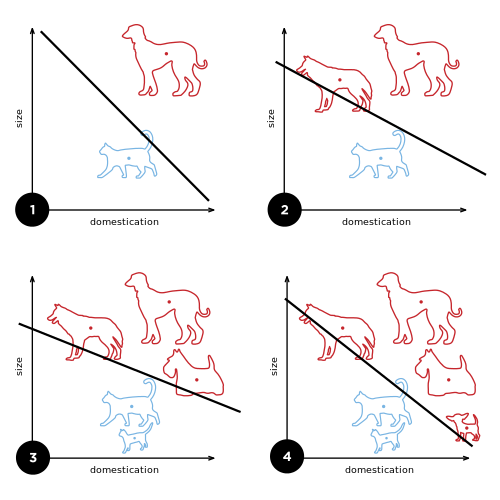
\includegraphics[width=0.9\textwidth]{images/Perceptron_example.svg.png}
       \end{figure}
          \end{column}
        \end{columns}
      \end{frame}

      \begin{frame}{Training von Neuronalen Netzen: Single-Layer-Perceptron}
        \begin{columns}
          \begin{column}{0.7\textwidth}
            \begin{itemize}

              \item Daraus folgt: \begin{align} 
                                  \nabla f(w) &= \left(  -\sum_{x \in F(w)} x_1,  -\sum_{x \in F(w)} x_2, ... ,  -\sum_{x \in F(w)} x_n   \right)
                                              &= -\sum_{x \in F(w)} x
                                  \end{align}
            \end{itemize}
          \end{column}
          \begin{column}{0.3\textwidth}
       \begin{figure}
       \centering
                   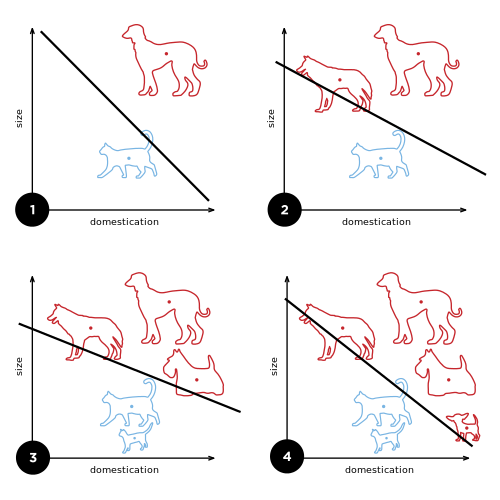
\includegraphics[width=0.9\textwidth]{images/Perceptron_example.svg.png}
       \end{figure}
          \end{column}
        \end{columns}
      \end{frame}

      \begin{frame}{Konstruktion von Neuronalen Netzen: Multi-Layer-Perceptron}
        \begin{columns}
          \begin{column}{0.7\textwidth}
            \begin{itemize}
              \item Wie können wir komplexere Formen als Geraden/Halbebenen abbilden?
              \item Kombination von vielen Halbebenen um Konvexe Formen zu erzeugen (logisches AND) 
              \item Mit noch einem weiteren Layer können wir ein logisches XOR und AND erzeugen
              \item insgesamt 3 Layer (input - hidden - output) reichen für beliebige Formen
              \item \emph{universal approximation theorem}
            \end{itemize}
          \end{column}
          \begin{column}{0.3\textwidth}
            \begin{figure}
              \centering
                          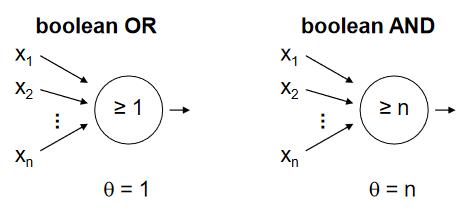
\includegraphics[width=0.9\textwidth]{images/OR_AND.png}
              \end{figure}
       \begin{figure}
       \centering
                   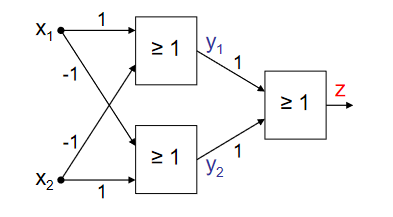
\includegraphics[width=0.9\textwidth]{images/XOR.png}
       \end{figure}
          \end{column}
        \end{columns}
      \end{frame}

      \begin{frame}{Training von Neuronalen Netzen: Multi-Layer-Perceptron}
        \begin{columns}
          \begin{column}{0.7\textwidth}
            \begin{itemize}
              \item Wie trainiert man nun ein solches Netz?
              \item Stelle eine Fehlerfunktion auf (Lossfunction)
              \begin{equation}
                f(w) = \sum_{x\in B} || g(w; x) - g^*(x) ||^2 \quad \rightarrow \text{  min  }
              \end{equation} 
              \item mit dem Output des Netzes $ g(w;x) $ und dem erwarteten Output $ g^*(x) $ 
              \item 
              \begin{align}
                 u^{(t+1)} &= u^t - \gamma \nabla_u f(w_t , u_t) \\
                 w^{(t+1)} &= w^t - \gamma \nabla_w f(w_t , u_t) \\
              \end{align}
              \item Problem: Unstetige Aktivierungsfunktion im hidden layer  $ a(x) = \begin{cases}1 & \text{if }\ x > \Theta,\\0 & \text{otherwise}\end{cases}$
              \item Lösung: Stetige und differenzierbare Aktivierungsfunktionen
            \end{itemize}
          \end{column}
          \begin{column}{0.3\textwidth}
            \begin{figure}
              \centering
                          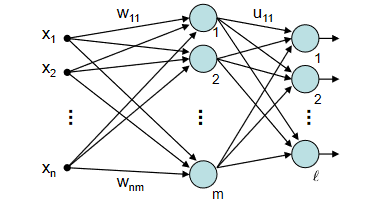
\includegraphics[width=0.9\textwidth]{images/MLP.png}
              \end{figure}
          \end{column}
        \end{columns}
      \end{frame}

      \begin{frame}{Training von Neuronalen Netzen: Multi-Layer-Perceptron}
        \begin{columns}
          \begin{column}{0.7\textwidth}
            \begin{itemize}
              \item
              \begin{equation}
                f(w) = \sum_{x\in B} || g(w; x) - g^*(x) ||^2 \quad \rightarrow \text{  min  }
              \end{equation} 
              \item mit dem Output des Netzes $ g(w;x) $ und dem erwarteten Output $ g^*(x) $ 
              \item 
              \begin{align}
                 u^{(t+1)} &= u^t - \gamma \nabla_u f(w_t , u_t) \\
                 w^{(t+1)} &= w^t - \gamma \nabla_w f(w_t , u_t) \\
              \end{align}
              \item $x_i$: Inputs 
              \item $y_j$: Werte nach dem ersten Layer
              \item $z_k$: Werte nach dem zweiten Layer
            \end{itemize}
          \end{column}
          \begin{column}{0.3\textwidth}
            \begin{figure}
              \centering
                          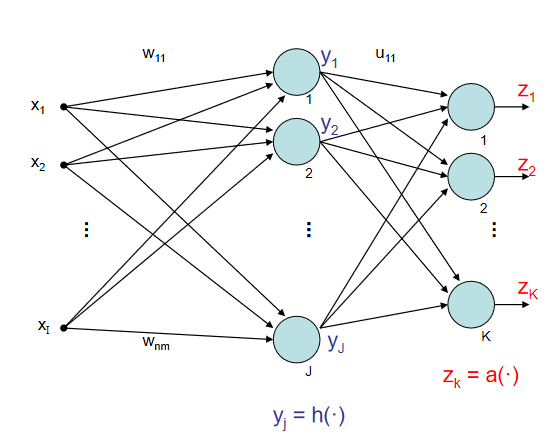
\includegraphics[width=0.9\textwidth]{images/MLP2.png}
              \end{figure}
          \end{column}
        \end{columns}
      \end{frame}

      \begin{frame}{Training von Neuronalen Netzen: Multi-Layer-Perceptron}
        \begin{columns}
          \begin{column}{1\textwidth}
            \begin{itemize}
              \item
              \begin{align*}
                y_j &= h \left( \sum_{i=1}^I w_{ij} \cdot x_i \right) = h(w_j'x) \\
                y_j &= a \left( \sum_{i=1}^I u_{jk} \cdot y_j \right) = a(w_k'y) \\
                    &= a \left(  \sum_{i=1}^I u_{jk} \cdot  h \left( \sum_{i=1}^I w_{ij} \cdot x_i \right)   \right)
              \end{align*} 
              \item mit dem Fehler des Inputs $x$:
              \begin{align*}
                f(w,u;x,z^*) &= \sum_{k=1}^K (z_k(x) -z^*_k(x) )^2 \\
                            &=  \sum_{k=1}^K [a(u_k y) - z_k*]^2
              \end{align*}
            \item analog zum SLP nutzen wir den Gradienten zur Minimierung des Fehlers
            \begin{align*}
              \nabla f(w,u) &= \sum_{x,z^* \in B} \nabla f(w, u; x,z^*) \\
              \frac{\partial f(w,u)}{\partial u_{jk}} &= \sum_{x,z^* \in B} \frac{\partial f(w,u;x,z^*)}{\partial u_{jk}} \\
              \frac{\partial f(w,u)}{\partial w_{ij}} &= \sum_{x,z^* \in B} \frac{\partial f(w,u;x,z^*)}{\partial w_{ij}} 
            \end{align*}
            \end{itemize}
          \end{column}
          %\begin{column}{0.3\textwidth}
          %  \begin{figure}
          %    \centering
          %                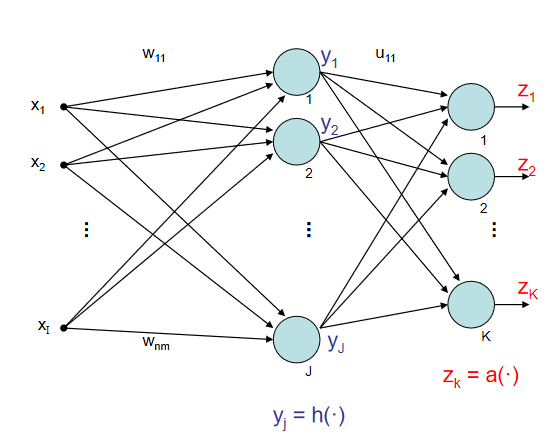
\includegraphics[width=0.9\textwidth]{images/MLP2.png}
          %    \end{figure}
          %\end{column}
        \end{columns}
      \end{frame}

      \begin{frame}{Training von Neuronalen Netzen: Multi-Layer-Perceptron}
        \begin{columns}
          \begin{column}{1\textwidth}
            \begin{itemize}
              \item analog zum SLP nutzen wir den Gradienten zur Minimierung des Fehlers
            \begin{align*}
              \nabla f(w,u) &= \sum_{x,z^* \in B} \nabla f(w, u; x,z^*) \\
              \frac{\partial f(w,u)}{\partial u_{jk}} &= \sum_{x,z^* \in B} \frac{\partial f(w,u;x,z^*)}{\partial u_{jk}} \\
              \frac{\partial f(w,u)}{\partial w_{ij}} &= \sum_{x,z^* \in B} \frac{\partial f(w,u;x,z^*)}{\partial w_{ij}} 
            \end{align*}
            \item mit den Sigmoid-Aktivierungsfunktionen:
            \begin{align*}
              a(x) = h(x) = \frac{1}{1+e^{-x}} \text{mit der Ableitung:  } \frac{\text{d}a(x)}{\text{dx}} = a(x) \cdot (1 - a(x))
            \end{align*}
            \item mit der Kettenregel für Ableitungen:
            \begin{equation*}
              [p(q(x))]´ = p´(q(x)) \cdot q´(x) 
            \end{equation*}
            \item ergibt sich für den Gradienten von $f$:
            \begin{align*}
              f(w,u;x,z^*) &= \sum_{k=1} ^K [a(u_k y) - z^*_k]^2 \\
              \frac{\partial f(w,u; x,z^*) }{ \partial u_{jk} } &= \sum_{x,z^* \in B} \frac{\partial f(w,u;x,z^*)}{\partial u_{jk}} \\
                                                            &= 2 [a(u´_k y)-z^*_k] \cdot a´(u´_k y) \cdot y_j \\
                                                            &= 2 [a(u´_k y)-z^*_k] \cdot a(u´_k y \cdot (1 - a(u´_k y)))\cdot y_j\\
                                                            &=  \underbrace{ 2 [z_k - z^*_k] \cdot z_k \cdot (1- z_k) }_\text{Fehlerterm $ \delta_k$} \cdot y_j \\
               \frac{\partial f(w,u; x,z^*)}{\partial w_{ij}} &= 2 \sum_{k=1} ^K (a(u´_k y) -z^*_k) \cdot a´(u´_k y) \cdot u_{jk} \cdot h´(w´_j x) x_i \\
                                                             &= 2 \sum_{k=1} ^K ( z_k -z^*_k) \cdot z_k \cdot (1-z_k) \cdot u_{jk} \cdot y_j (1-y_j) x_i \\                                                            
                                                             &= x_i y_j (1-y_j)  \underbrace{2 \sum_{k=1} ^K ( z_k -z^*_k) \cdot z_k \cdot (1-z_k) }_\text{Fehlerterm $ \delta_i$} \cdot u_{jk} \cdot y_j 
            \end{align*}
            \end{itemize}
          \end{column}
          %\begin{column}{0.3\textwidth}
          %  \begin{figure}
          %    \centering
          %                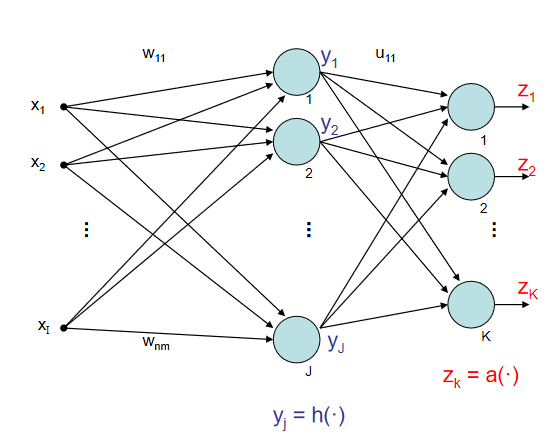
\includegraphics[width=0.9\textwidth]{images/MLP2.png}
          %    \end{figure}
          %\end{column}
        \end{columns}
      \end{frame}
      \begin{frame}{Training von Neuronalen Netzen: Multi-Layer-Perceptron}
        \begin{columns}
          \begin{column}{1\textwidth}
            \begin{itemize}

            \item ergibt sich für den Gradienten von $f$:
            \begin{align*}
              f(w,u;x,z^*) &= \sum_{k=1} ^K [a(u_k y) - z^*_k]^2 \\
              \frac{\partial f(w,u; x,z^*) }{ \partial u_{jk} } &= \sum_{x,z^* \in B} \frac{\partial f(w,u;x,z^*)}{\partial u_{jk}} \\
                                                            &= 2 [a(u´_k y)-z^*_k] \cdot a´(u´_k y) \cdot y_j \\
                                                            &= 2 [a(u´_k y)-z^*_k] \cdot a(u´_k y \cdot (1 - a(u´_k y)))\cdot y_j\\
                                                            &=  \underbrace{ 2 [z_k - z^*_k] \cdot z_k \cdot (1- z_k) }_\text{Fehlerterm $ \delta_k$} \cdot y_j \\
               \frac{\partial f(w,u; x,z^*)}{\partial w_{ij}} &= 2 \sum_{k=1} ^K (a(u´_k y) -z^*_k) \cdot a´(u´_k y) \cdot u_{jk} \cdot h´(w´_j x) x_i \\
                                                             &= 2 \sum_{k=1} ^K ( z_k -z^*_k) \cdot z_k \cdot (1-z_k) \cdot u_{jk} \cdot y_j (1-y_j) x_i \\                                                            
                                                             &= x_i y_j (1-y_j)  \underbrace{2 \sum_{k=1} ^K ( z_k -z^*_k) \cdot z_k \cdot (1-z_k) }_\text{Fehlerterm $ \delta_i$} \cdot u_{jk} \cdot y_j 
            \end{align*}
            \end{itemize}
          \end{column}
          %\begin{column}{0.3\textwidth}
          %  \begin{figure}
          %    \centering
          %                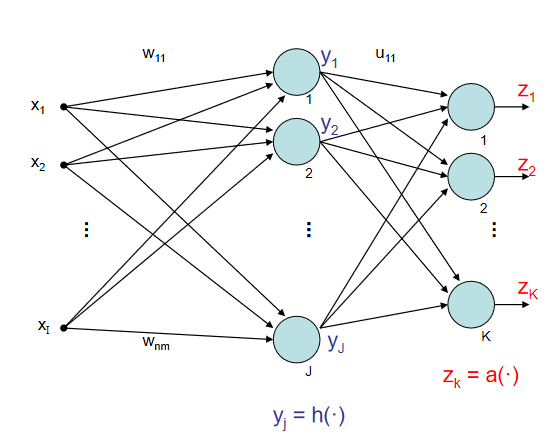
\includegraphics[width=0.9\textwidth]{images/MLP2.png}
          %    \end{figure}
          %\end{column}
        \end{columns}
      \end{frame}

      \begin{frame}{ Verallgemeinerung Training von Neuronalen Netzen: M-Layer-Perceptron}
        \begin{columns}
          \begin{column}{1\textwidth}
            \begin{itemize}
              \item bei einem Neuronalen Netz mi $L$ Layern $S_1, S_2 , ... , S_L$
              \item den Gewichten $w_{ij}$ in der Matrix $W$
              \item dem output eines Neurons $o_j$
              \item ist der Fehlerterm: 
            \begin{equation*}
              \delta_j = \begin{cases} o_j \cdot (1-o_j) \cdot  (o_j -z_j*) & \text{if }\ j \in S_L, \text{output Neuron} \\ o_j \cdot (1-o_j) \cdot \sum_{k \in S_{m+1}} \delta_k \cdot w_{jk} & \text{if } j \in S_m \text{and } m<L \end{cases}
            \end{equation*}
            \item Der Korrekturterm für die einzelnen Gewichte ist dann:
            \begin{equation}
              w_{ij}^{(t+1)} = w_{ij}^{t} - \gamma \cdot o_i \cdot \delta_j 
            \end{equation}
            \end{itemize}
          \end{column}
          %\begin{column}{0.3\textwidth}
          %  \begin{figure}
          %    \centering
          %                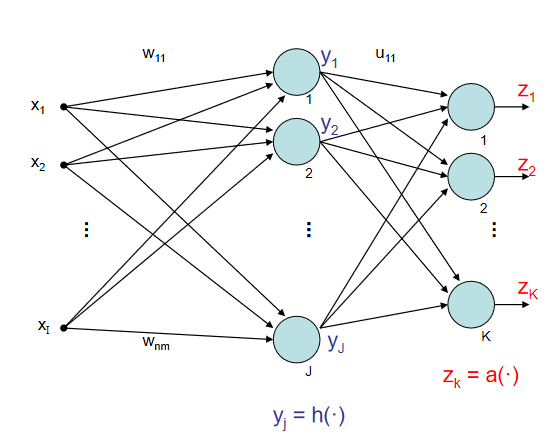
\includegraphics[width=0.9\textwidth]{images/MLP2.png}
          %    \end{figure}
          %\end{column}
        \end{columns}
      \end{frame}

      \begin{frame}{ Verallgemeinerung Training von Neuronalen Netzen: M-Layer-Perceptron}
        \begin{columns}
          \begin{column}{1\textwidth}
            \begin{itemize}
              \item Weitere Trainingsalgorithmen:
              \item Backpropagation with Momentum \rightarrow Berücksichtigung der voherigen Gewichtsänderungen
              \item ADAM (Adaptive Moment Estimation)
              \begin{align*}
                m_w ^ {(t+1)} &\leftarrow \beta_1 m_w ^ {(t)} + (1 - \beta_1) \nabla _w L ^ {(t)}\\
                v_w ^ {(t+1)} &\leftarrow \beta_2 v_w ^ {(t)} + (1 - \beta_2) (\nabla _w L ^ {(t)} )^2\\
                \hat{m}_w &= \frac{m_w ^ {(t+1)}}{1 - \beta_1}\\
                \hat{v}_w &= \frac{ v_w ^ {(t+1)}}{1 - \beta_2}\\         
                w ^ {(t+1)} &\leftarrow w ^ {(t)} - \gamma \frac{\hat{m}_w}{\sqrt{\hat{v}_w} + \epsilon}
              \end{align*}
              \item mit einer kleinen Zahl $\epsilon$ und Skalierungsfaktoren $\beta_i$
            \end{itemize}
          \end{column}
          % \begin{column}{0.3\textwidth}
          %   \begin{figure}
          %     \centering
          %                 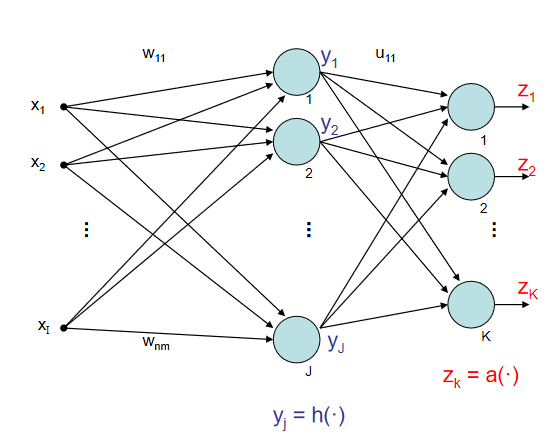
\includegraphics[width=0.9\textwidth]{images/MLP2.png}
          %     \end{figure}
          % \end{column}
        \end{columns}
      \end{frame}

      \begin{frame}{ How Deep is your Network?}
        \begin{columns}
          \begin{column}{0.6\textwidth}
            \begin{itemize}
              \item bei mehr als 3 Layern wird häufig von "Deep Learning" gesprochen
              \item Wieso nutzen wir mehr als 3 Layer?
              \item Viele Machine Learning Algorithmen leben von Feature Engineering
              \item eine naive Vorstellung:
              \item wir haben $L$ Layer von denen 3 Layer unseren endgültigen Klassifikator bilden
              \item Die restlichen $L-3$ Layer "erzeugen" Feature
              \item Nachteile: Training von vielen Layern ist "teuer"
              \item Verschwindende Gradienten bei der Sigmoid Funktion
            \end{itemize}
          \end{column}
           \begin{column}{0.4\textwidth}
             \begin{figure}
               \centering
                           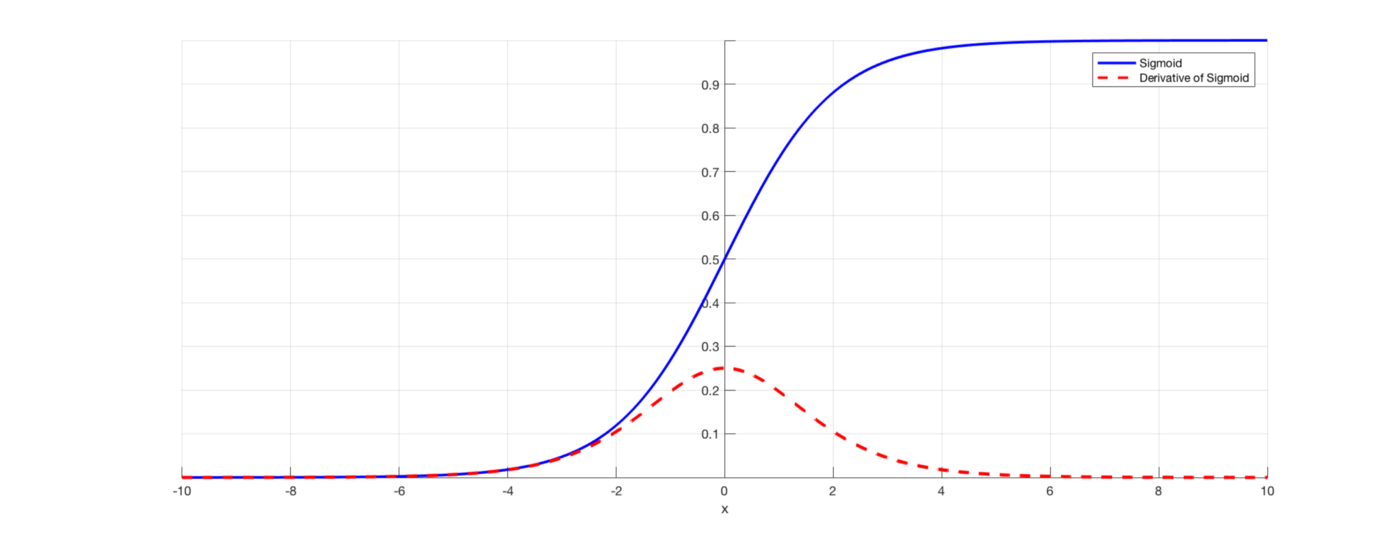
\includegraphics[width=0.9\textwidth]{images/sigmoid.png}
               \end{figure}
           \end{column}
        \end{columns}
      \end{frame}

      \begin{frame}{Häufige Aktivierungsfunktionen}
        \begin{columns}
          \begin{column}{0.5\textwidth}
            \begin{figure}
              \centering
                          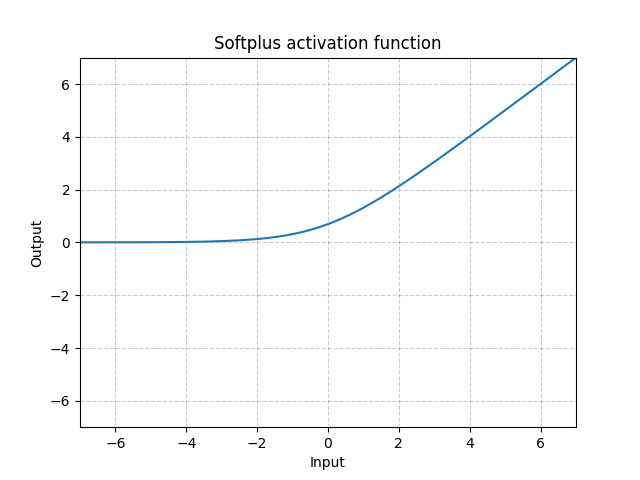
\includegraphics[width=0.9\textwidth]{images/Softplus.png}
              \end{figure}
          \end{column}
           \begin{column}{0.5\textwidth}
             \begin{figure}
               \centering
                           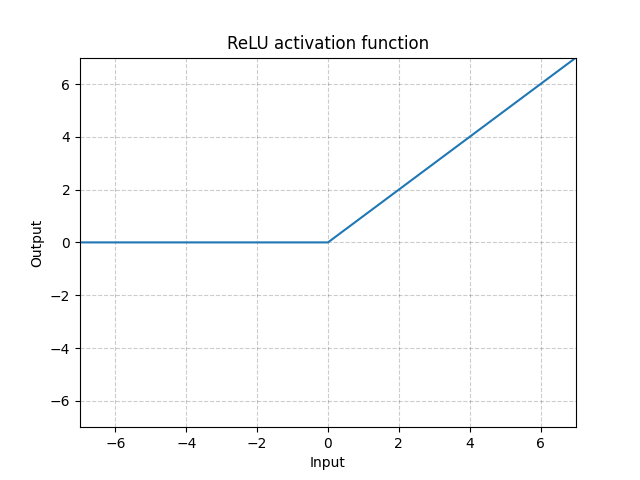
\includegraphics[width=0.9\textwidth]{images/ReLU.png}
               \end{figure}
           \end{column}
        \end{columns}
      \end{frame}

      
      \begin{frame}{Weitere Netzwerk Architekturen}
        \begin{columns}
          \begin{column}{0.6\textwidth}
            \begin{itemize}
              \item spezielle Datenstrukturen profitieren von speziellen Architekturen \newline 
              \item Bilderkennung \rightarrow Convolutional Neural Network (CNN) \newline 
              \item sequentielle Daten \rightarrow Recurrent Neural Networks (RNN) \newline 
              \item im speziellen um Kausalität/Kontext herzustellen \rightarrow Long Short Term Memory (LSTM) \newline
            \end{itemize}
          \end{column}
           \begin{column}{0.4\textwidth}
             \begin{figure}
               \centering
                           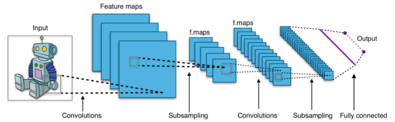
\includegraphics[width=0.9\textwidth]{images/CNN.png}
               \end{figure}
               \begin{figure}
                \centering
                            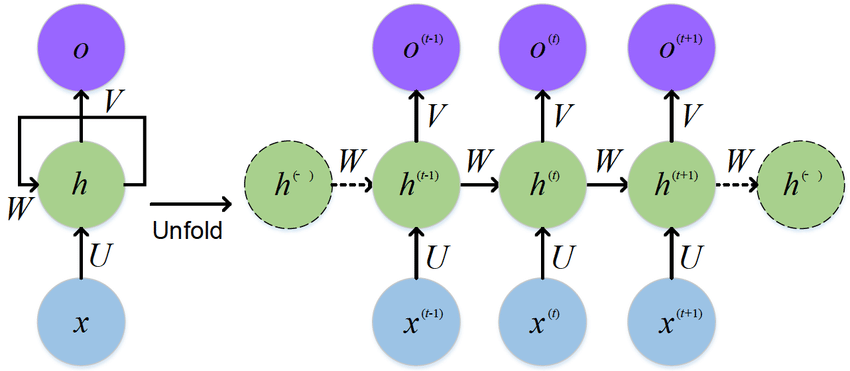
\includegraphics[width=0.9\textwidth]{images/RNN.png}
                \end{figure}
           \end{column}
        \end{columns}
      \end{frame}

      \begin{frame}{Spezielle Netzwerkarchitekturen: CNN}
        \begin{columns}
          \begin{column}{0.6\textwidth}
            \begin{itemize}
              \item Convolution := Faltung \newline 
              \item Verringerung der Dimensionalität durch Zusammenfassen von aneinanderliegenden Pixeln \newline 
              \item Zusammenfassen von Informationen \newline 
              \item Erzeugt 2D-Feature \newline 
              \item MLP klassifiziert anschließend mit diesen Features \newline
            \end{itemize}
          \end{column}
           \begin{column}{0.4\textwidth}
             \begin{figure}
               \centering
                           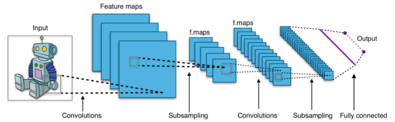
\includegraphics[width=0.9\textwidth]{images/CNN.png}
               \end{figure}
               \begin{figure}
                \centering
                            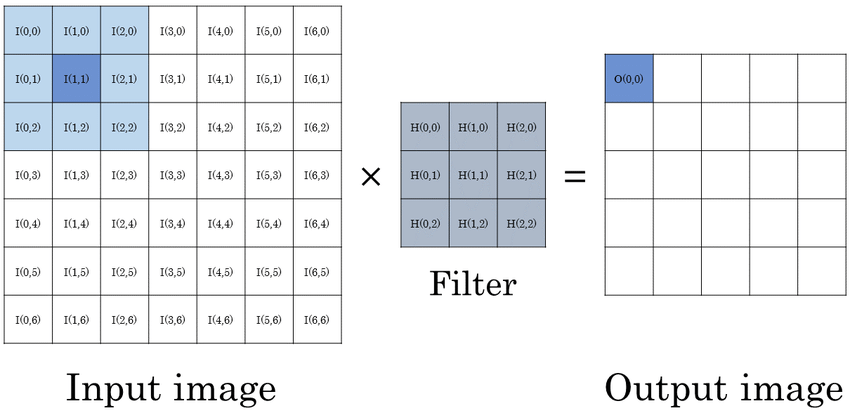
\includegraphics[width=0.9\textwidth]{images/convolution.png}
                \end{figure}
           \end{column}
        \end{columns}
      \end{frame}

      \begin{frame}{Spezielle Netzwerkarchitekturen: CNN}
        \begin{columns}
          \begin{column}{0.5\textwidth}
            \begin{itemize}
              \item Anschaulich: Formen werden erkannt \newline 
              \item Katzenohren sind anders als Hundeohren \newline 
              \item Verallgemeinerbar für andere Objektklassifizierungen \newline
            \end{itemize}
          \end{column}
           \begin{column}{0.5\textwidth}
             \begin{figure}
               \centering
                           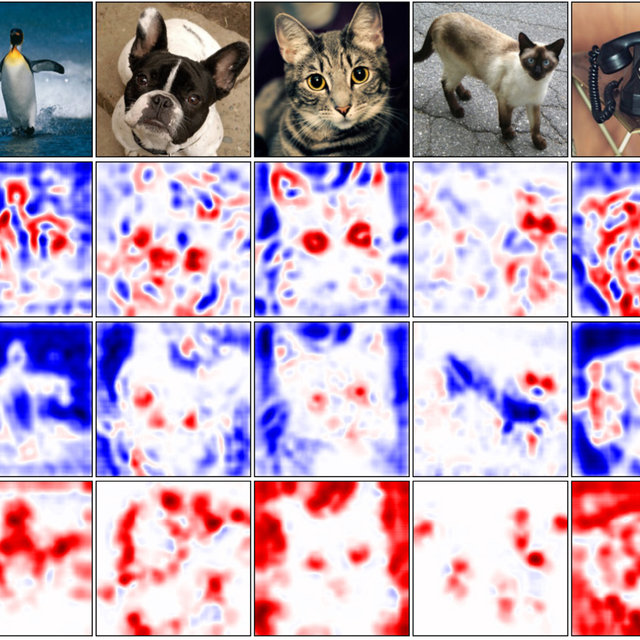
\includegraphics[width=0.9\textwidth]{images/featuremaps.jpg}
               \end{figure}

           \end{column}
        \end{columns}
      \end{frame}

      \begin{frame}{Spezielle Netzwerkarchitekturen: RNN}
        \begin{columns}
          \begin{column}{0.6\textwidth}
            \begin{itemize}
              \item Anschaulich: Schleife in Netzwerk "merkt" sich voherige Zustände \newline 
              \item funktioniert für kurze Zeiträume \newline 
              \item Entfaltung eines RNN \rightarrow viele zu trainierende Gewichte \newline 
              \item Problem: langfristige Zusammenhänge werden nicht erfasst \newline 
              \item Problem: Verschwindende Gradienten
            \end{itemize}
          \end{column}
           \begin{column}{0.4\textwidth}
             \begin{figure}
               \centering
                           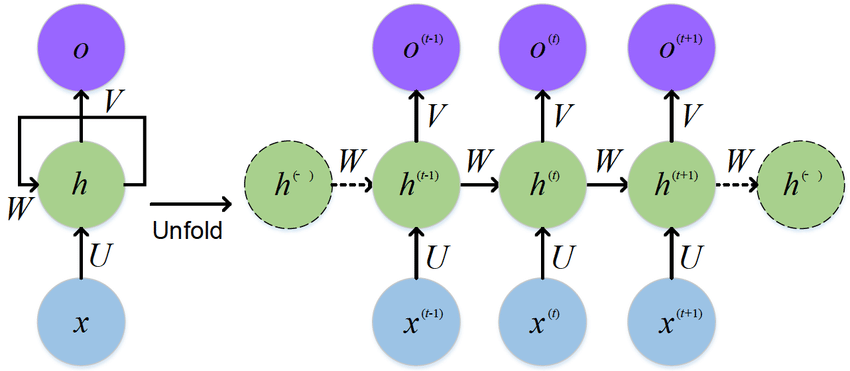
\includegraphics[width=0.9\textwidth]{images/RNN.png}
               \end{figure}

           \end{column}
        \end{columns}
      \end{frame}     
      
      \begin{frame}{Spezielle Netzwerkarchitekturen: LSTM}
        \begin{columns}
          \begin{column}{0.6\textwidth}
            \begin{itemize}
              \item Gesamtdarstellung eines "entfalteten" LSTM \newline 
              \item zum Cell State $C$ werden Infromationen hinzugefügt \newline 
              
              
            \end{itemize}
          \end{column}
           \begin{column}{0.4\textwidth}
             \begin{figure}
               \centering
                           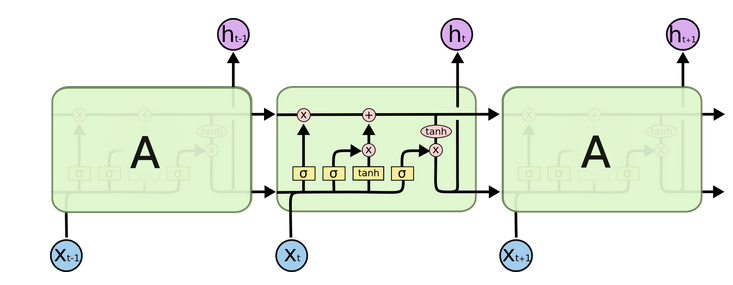
\includegraphics[width=0.9\textwidth]{images/LSTM_1.png}
               \end{figure}
               \begin{figure}
                \centering
                            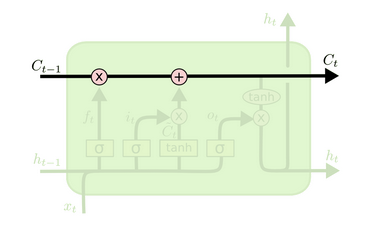
\includegraphics[width=0.9\textwidth]{images/LSTM_2.png}
                \end{figure}

           \end{column}
        \end{columns}
      \end{frame}
      
            
      \begin{frame}{Spezielle Netzwerkarchitekturen: LSTM}
        \begin{columns}
          \begin{column}{0.6\textwidth}
            \begin{itemize}              
              \item Forget Gate "entscheidet" mit einer Sigmoid-Funktion $\sigma$ ob ein Vorheriger Zustand vergessen wird \newline
              \item Input Gate entscheidet mit dem voherigen hidden state ob ein neues Ereignis weitergegeben wird
            \end{itemize}
          \end{column}
           \begin{column}{0.4\textwidth}
             \begin{figure}
               \centering
                           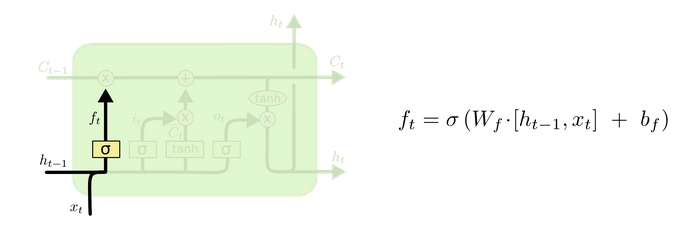
\includegraphics[width=0.9\textwidth]{images/LSTM_3.png}
               \end{figure}
               \begin{figure}
                \centering
                            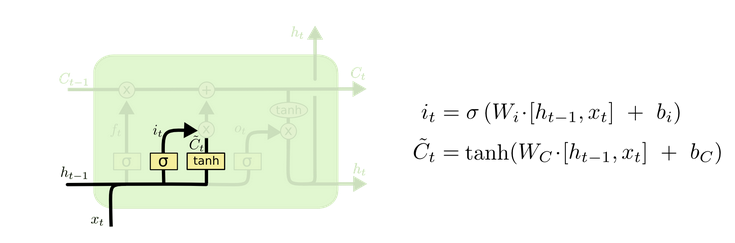
\includegraphics[width=0.9\textwidth]{images/LSTM_4.png}
                \end{figure}
            

           \end{column}
        \end{columns}
      \end{frame} 

      \begin{frame}{Spezielle Netzwerkarchitekturen: LSTM}
        \begin{columns}
          \begin{column}{0.6\textwidth}
            \begin{itemize}
             
              \item Update des alten Cell states mithilfe des alten und neuen Zustandes \newline 
              \item Output der LSTM Zelle und Erzeugung des neuen hidden states \newline 
            \end{itemize}
          \end{column}
           \begin{column}{0.4\textwidth}
            
               \begin{figure}
                \centering
                            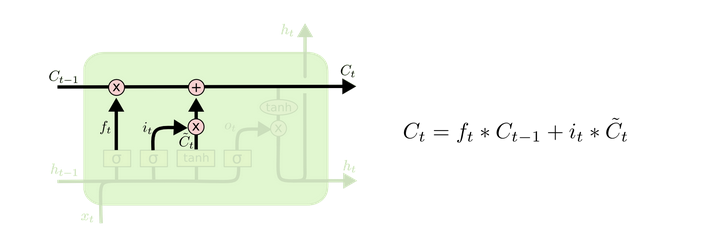
\includegraphics[width=0.9\textwidth]{images/LSTM_5.png}
                \end{figure}
                \begin{figure}
                  \centering
                              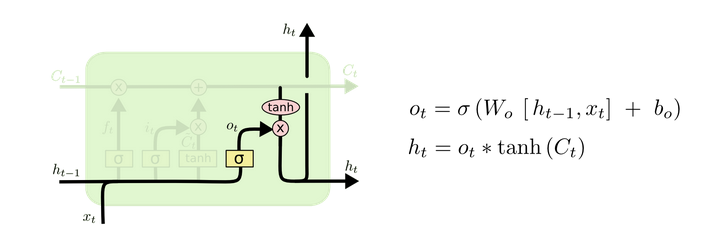
\includegraphics[width=0.9\textwidth]{images/LSTM_6.png}
                  \end{figure}

           \end{column}
        \end{columns}
      \end{frame} 


      \begin{frame}{Spezielle Netzwerkarchitekturen: Unsupervised Learning}
        \begin{columns}
          \begin{column}{0.6\textwidth}
            \begin{itemize}
              \item Autoencoder bzw. Encoder-Decoder Netzwerke \newline
              \item Versuch den Input wieder zu rekonstruieren \rightarrow Interessant für unsupervised anomaly detection \newline 
              \item Generative Netzwerk \newline
              \item Möglichkeit aus "Noise" komplexe echt aussehende Daten zu erzeugen \rightarrow mögliche Beschleunigung von (FE-)Simulationen
            \end{itemize}
          \end{column}
           \begin{column}{0.4\textwidth}
             \begin{figure}
               \centering
                           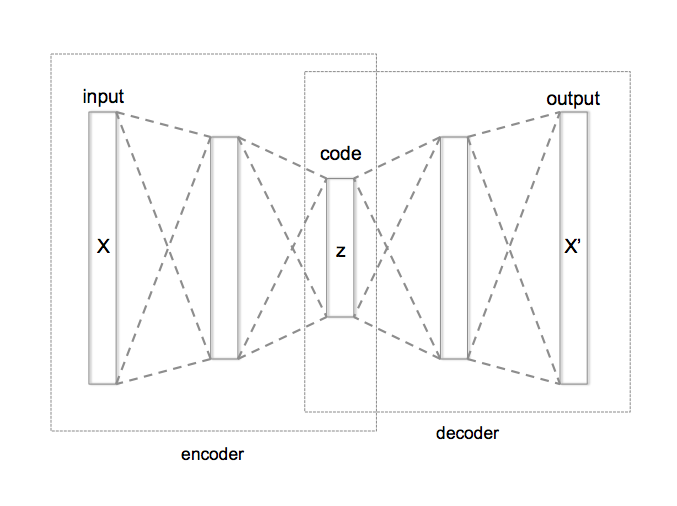
\includegraphics[width=0.9\textwidth]{images/Autoencoder.png}
               \end{figure}
               \begin{figure}
                \centering
                            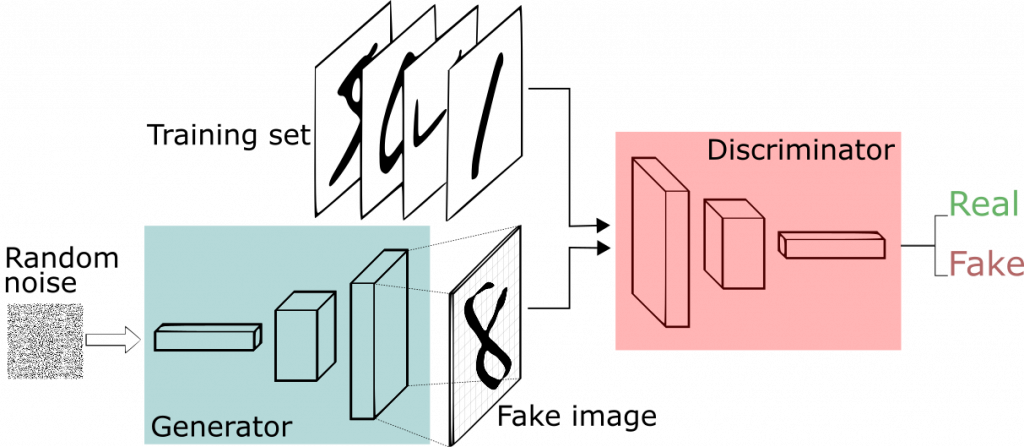
\includegraphics[width=0.9\textwidth]{images/GAN.png}
                \end{figure}
            \end{column}
        \end{columns}
      \end{frame} 

      \begin{frame}{Was ist Predictive Maintenance?}
      \begin{columns}
        \begin{column}{1\textwidth}
          Grundlegende Ziele
          \begin{itemize}
            \item Prozessüberwachung und eventuelle Steuerung \newline
            \item Vorhersagen von Maschinen/Produktionsausfällen\newline 
            \item Hilfe/Unterstüzung bei der Wartungsplanung \newline 
            \item Klassifikation von Fehlerzuständen \newline 
            \item ...
          \end{itemize}
        \end{column}
        % \begin{column}{0.4\textwidth}
        %   \begin{figure}
        %     \centering
        %      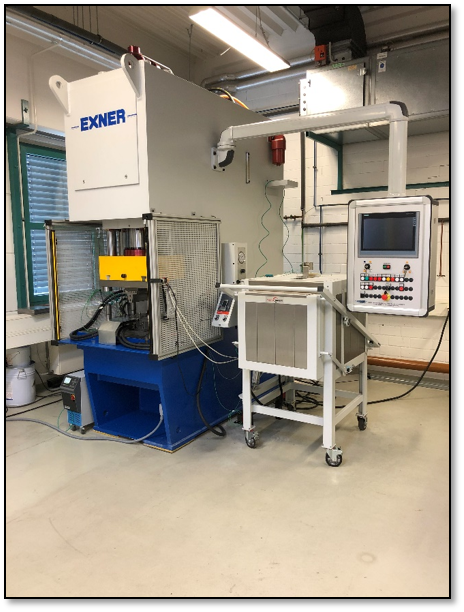
\includegraphics[width=0.6\textwidth]{images/anlage.png}
        %   \end{figure}
        % \end{column}
      \end{columns}
        \end{frame}
    

        \begin{frame}{Was ist Predictive Maintenance?}
          \begin{columns}
            \begin{column}{1\textwidth}
              \begin{itemize}
                \item PM ist als Teilbereich der Industrie 4.0 zu verstehen \newline
                \item (Nah-) Echtzeitdatenanalysen sollen Bedarfsgerechte Wartung ermöglichen \newline
                \item Großes Potential der Kosteneinsparung \newline
              \end{itemize}
            \end{column}
            % \begin{column}{0.4\textwidth}
            %   \begin{figure}
            %     \centering
            %      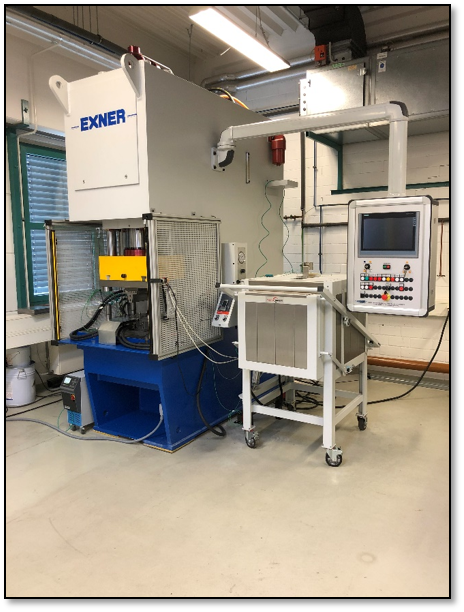
\includegraphics[width=0.6\textwidth]{images/anlage.png}
            %   \end{figure}
            % \end{column}
          \end{columns}
            \end{frame}

            \begin{frame}{Fallbeispiel: Vollautomatisierte Produktionszelle}
              \begin{columns}
                \begin{column}{1\textwidth}
                  \begin{itemize}
                    \item Automatisierungstechnik liefert Prozessdaten \newline
                    \item zusätzliche Sensorik liefert mehr Daten \newline
                    \item Ein Trend in den Daten deutet auf einen zukünftigen Fehler hin \newline
                    \item Der Fehler wird klassifiziert und eine Handlungsanweisung wird herausgegeben \newline
                    \item Der Fehler kann, bevor er größere Schäden, oder Produktionsausfälle behoben werden \newline
                    \item Wielche Schritte sind dafür Notwendig?
                  \end{itemize}
                \end{column}
                % \begin{column}{0.4\textwidth}
                %   \begin{figure}
                %     \centering
                %      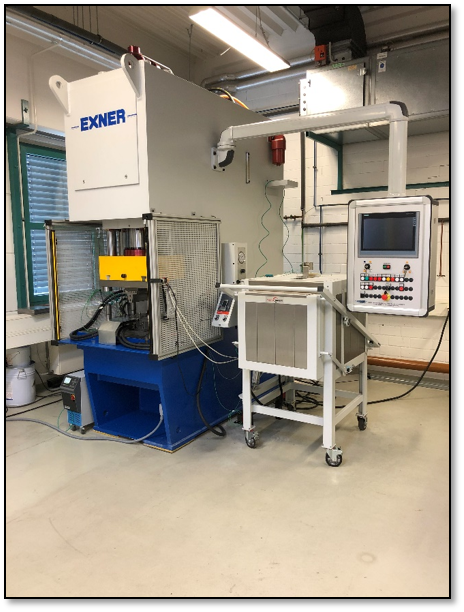
\includegraphics[width=0.6\textwidth]{images/anlage.png}
                %   \end{figure}
                % \end{column}
              \end{columns}
                \end{frame}

                \begin{frame}{Fallbeispiel: Vollautomatisierte Produktionszelle -- Outline}
                  \begin{columns}
                    \begin{column}{1\textwidth}
                      Ausgangslage Industrie 3.0
                      \begin{itemize}
                        \item Automatisierungstechnik existiert und Daten stehen der Anlagensteuerung zur Verfügung\newline
                        \item Wie werden die Daten weiterverarbeitet? Haben Sie Beispiele aus Ihrem Unternehmen? \newline
                        \item eine Möglichkeit: Auslesen der Daten über eine OPC-UA Schnittstelle \newline
                        \item Weiterleitung dieser Daten über ein schnelle und skalierbare Schnittstelle (MQTT, ApacheKafka, ...) \newline
                        \item Empfang dieser Daten auf einem Datenbankserver (MariaDB, TimeseriesDB, ApacheDruid, ...) \newline
                        \item Durchführung von Echtzeitanalysen auf einem Edge-Computer, oder in der Cloud
                      \end{itemize}
                    \end{column}
                    % \begin{column}{0.4\textwidth}
                    %   \begin{figure}
                    %     \centering
                    %      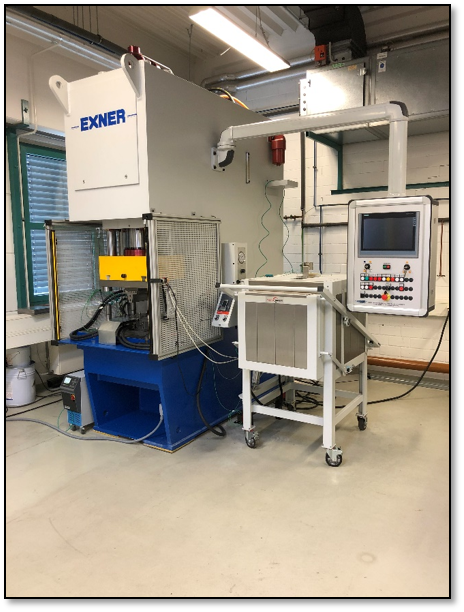
\includegraphics[width=0.6\textwidth]{images/anlage.png}
                    %   \end{figure}
                    % \end{column}
                  \end{columns}
                    \end{frame}

                    \begin{frame}{Fallbeispiel: Vollautomatisierte Produktionszelle -- Warmumformanlage}
                      \begin{columns}
                        \begin{column}{1\textwidth}
                          \begin{itemize}
                            \item Umformung und gleichzeitige Härtung von Stahl im Automobilleichtbau \newline
                            \item Probleme:
                            \item Komplexe Wirkzusammenhänge während des Prozesses \newline
                            \item Verlust von Know-How bei Standortwechseln der Produktion \newline
                            \item Langwierige Prüfverfahren zur Qualitätssicherung \rightarrow hohes Schadenspotential bei unentdeckten Fehlern \newline
                          \end{itemize}
                        \end{column}
                         \begin{column}{0.4\textwidth}
                           \begin{figure}
                             \centering
                              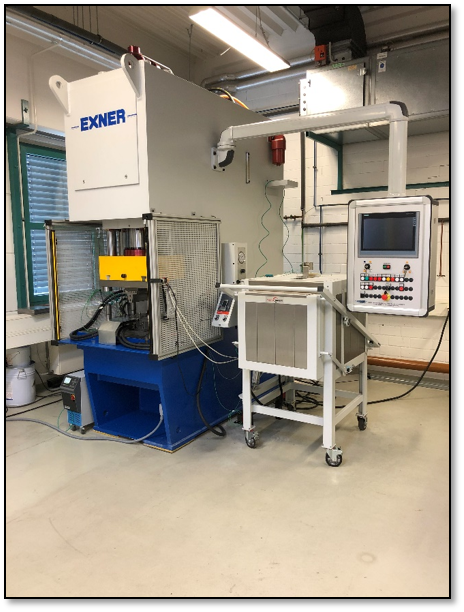
\includegraphics[width=0.6\textwidth]{images/anlage.png}
                           \end{figure}
                         \end{column}
                      \end{columns}
                        \end{frame}

                    \begin{frame}{Visualisierung eines möglichen Backends}
                      \begin{columns}
                        \begin{column}{1\textwidth}
                           \begin{figure}
                             \centering
                              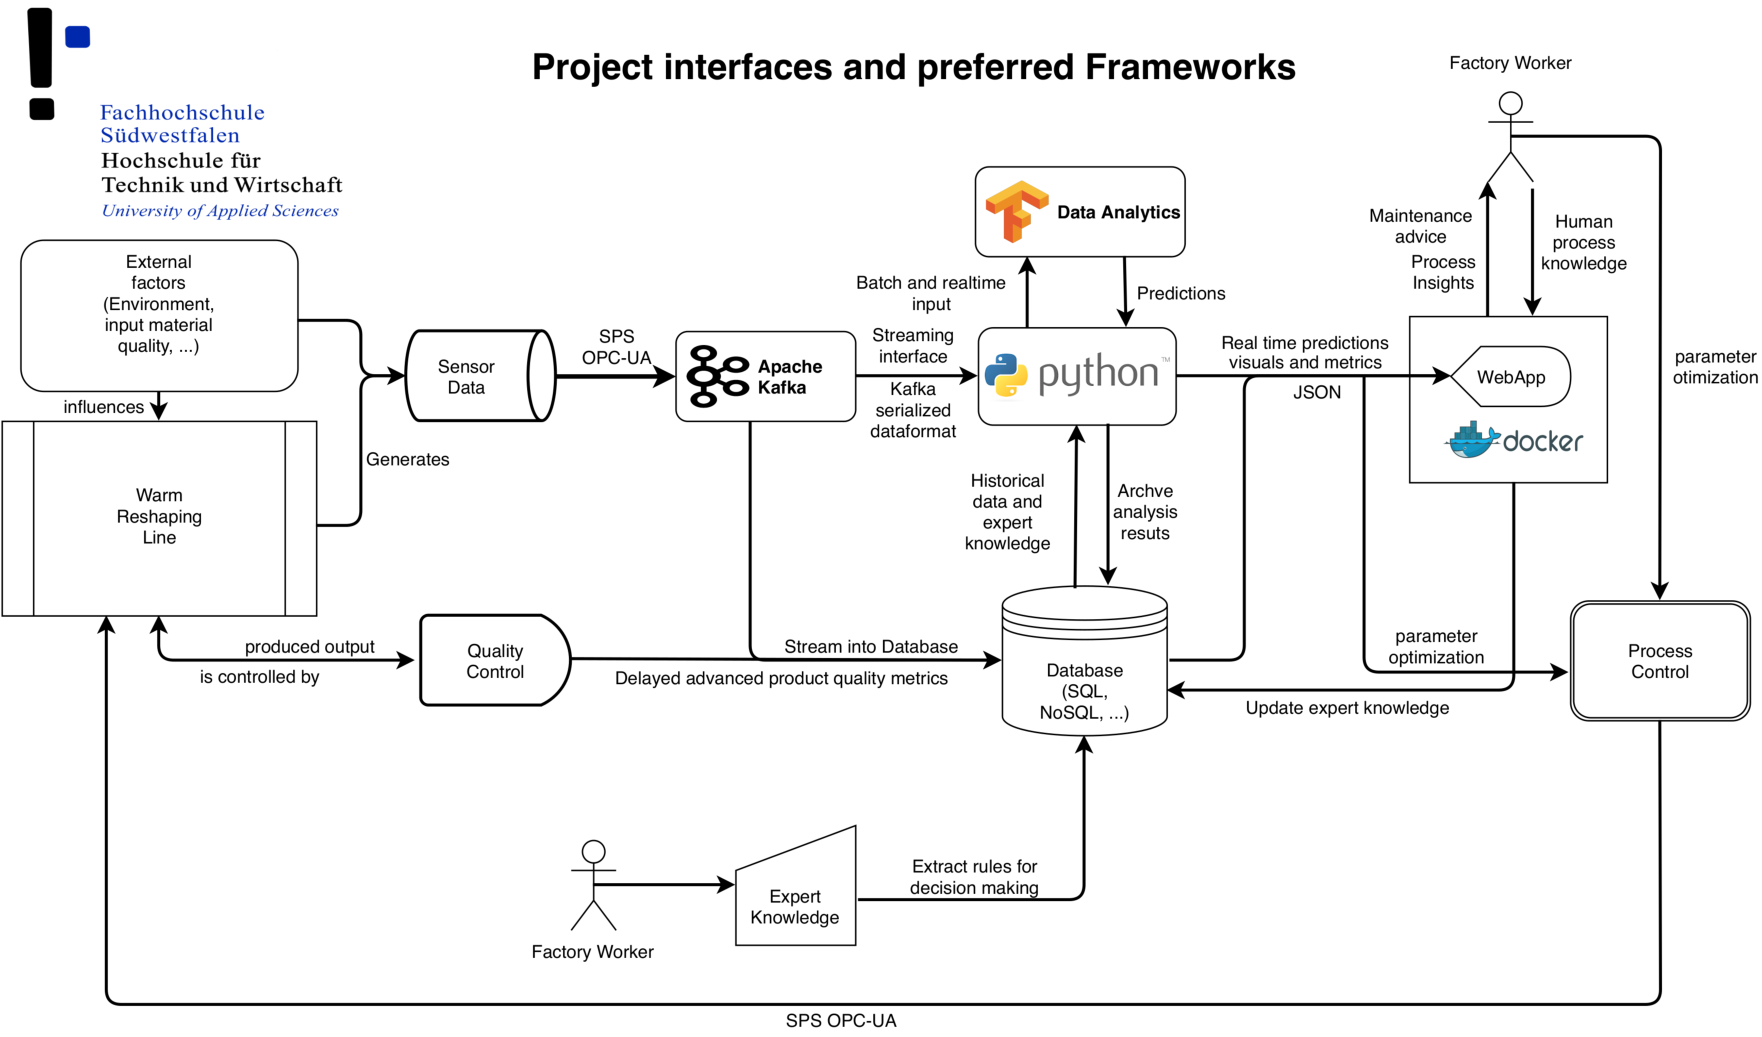
\includegraphics[width=0.6\textwidth]{images/process_v1_new.pdf}
                           \end{figure}
                         \end{column}
                      \end{columns}
                        \end{frame}

            \begin{frame}{Fallbeispiel: Vollautomatisierte Produktionszelle -- Datensammlung}
                          \begin{columns}
                            \begin{column}{1\textwidth}
                              \begin{itemize}
                                \item Prozessdaten werden mit einer OPC-UA Schnittstelle aus der übergeordneten Steuerung gelesen  \newline
                                \item Die Qualitätssicherung liefert verzögert Daten über die gefertigten Bauteile  \newline
                                \item Experten geben Know-How über den Prozess in einer strukturiterten Form einer FMEA (Failure Mode and Effects Analysis) ein \newline
                              \end{itemize}
                            \end{column}
                            % \begin{column}{0.4\textwidth}
                            %   \begin{figure}
                            %     \centering
                            %      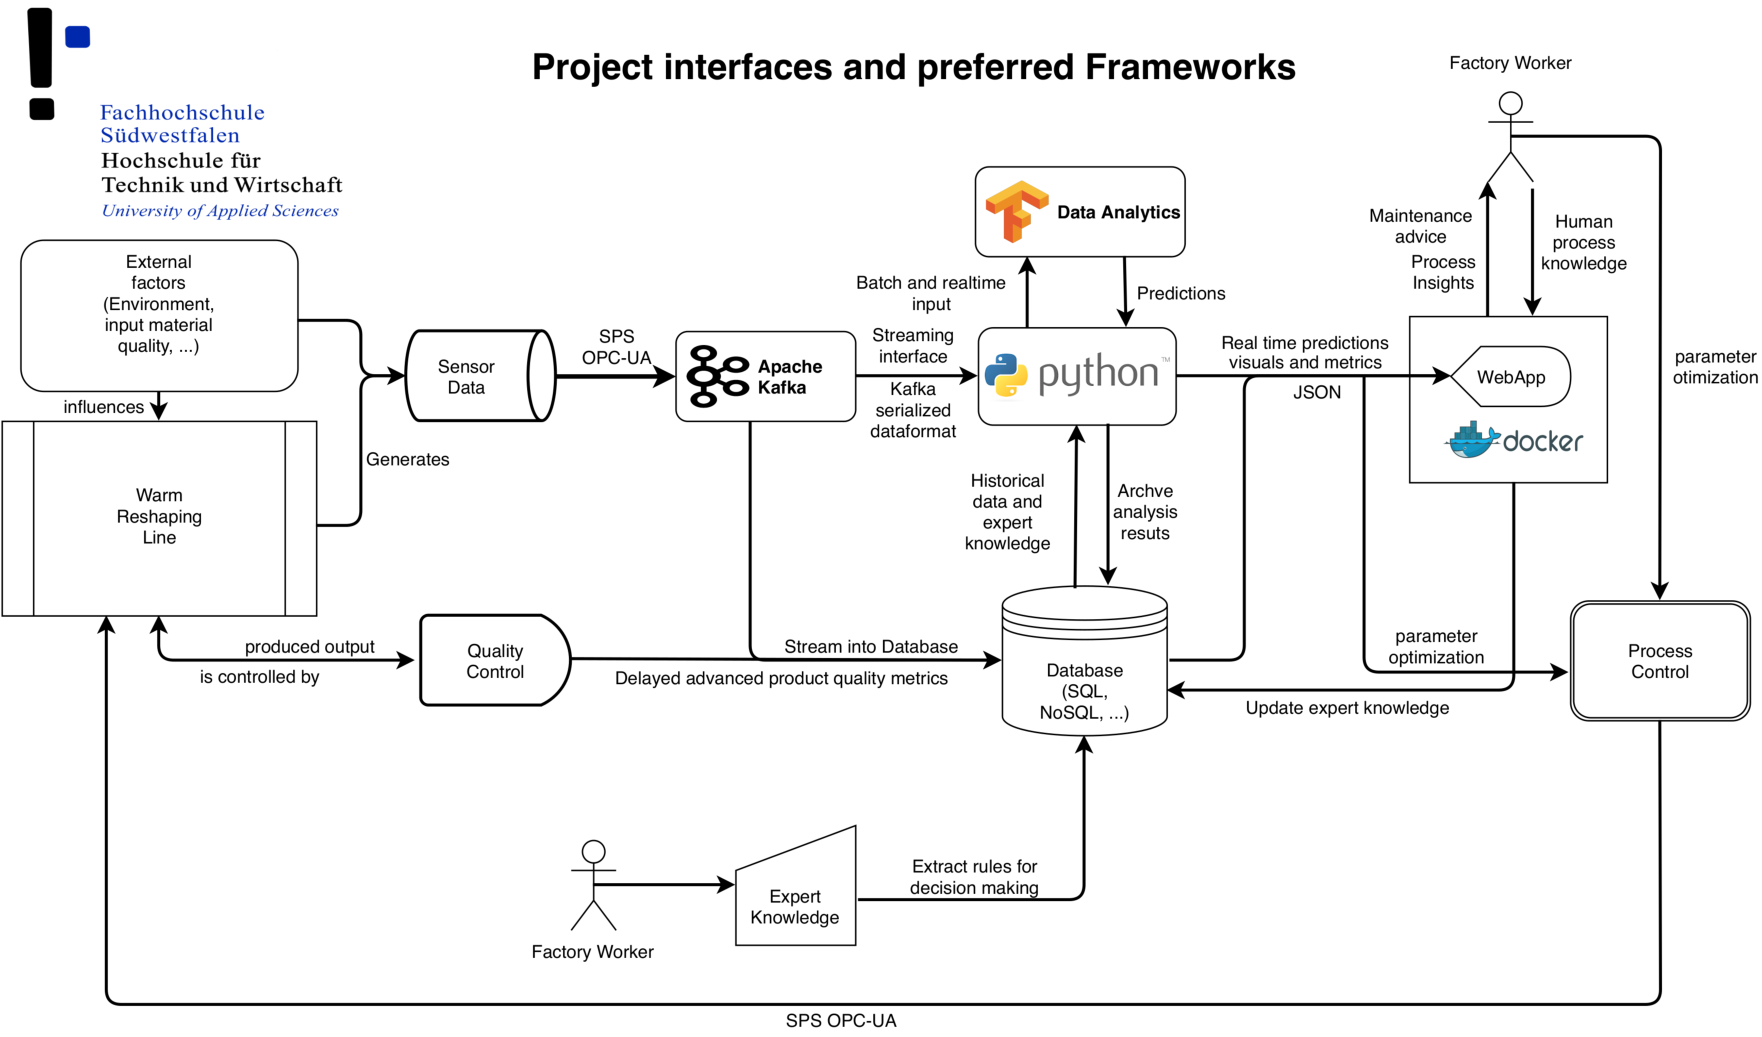
\includegraphics[width=0.4\textwidth]{images/process_v1_new.pdf}
                            %   \end{figure}
                            % \end{column}
                          \end{columns}
               \end{frame}   
          
          \begin{frame}{Fallbeispiel: Vollautomatisierte Produktionszelle -- Erste Datenverarbeitung mit einem Broker System}
                      \begin{columns}
                        \begin{column}{0.6\textwidth}
                          \begin{itemize}
                            \item Die Daten aus der Anlagensteuerung werden mit einem "Producer" an einen Broker geschickt, der den Datenstrom verwaltet \newline
                            \item Ein Brokersystem wie ApacheKafka oder MQTT kontrolliert den Datenfluss \newline
                            \item Clients können dem Broker "folgen" (subscriben) \newline
                            \item Ein sogenannter Consumer erhält diesen nun bei jedem neuen erzeugten Datenpunkt \newline
                            \item Diese Datenpunkte können dann mit einem Machine Learning Framework (sci-kit-learn, TensorFlow, PyTorch) analysiert werden \newline
                            \item Vorteil: Parallelisierung des Datenflusses möglich
                            \item Gleichzeitiges Speichern der Daten in einer Datenbank und Echtzeitverarbeitung im Datenanalyse Framework und darstellung auf einem Dashboard \newline  
                          \end{itemize}
                        \end{column}
                        % \begin{column}{0.4\textwidth}
                        %   \begin{figure}
                        %     \centering
                        %      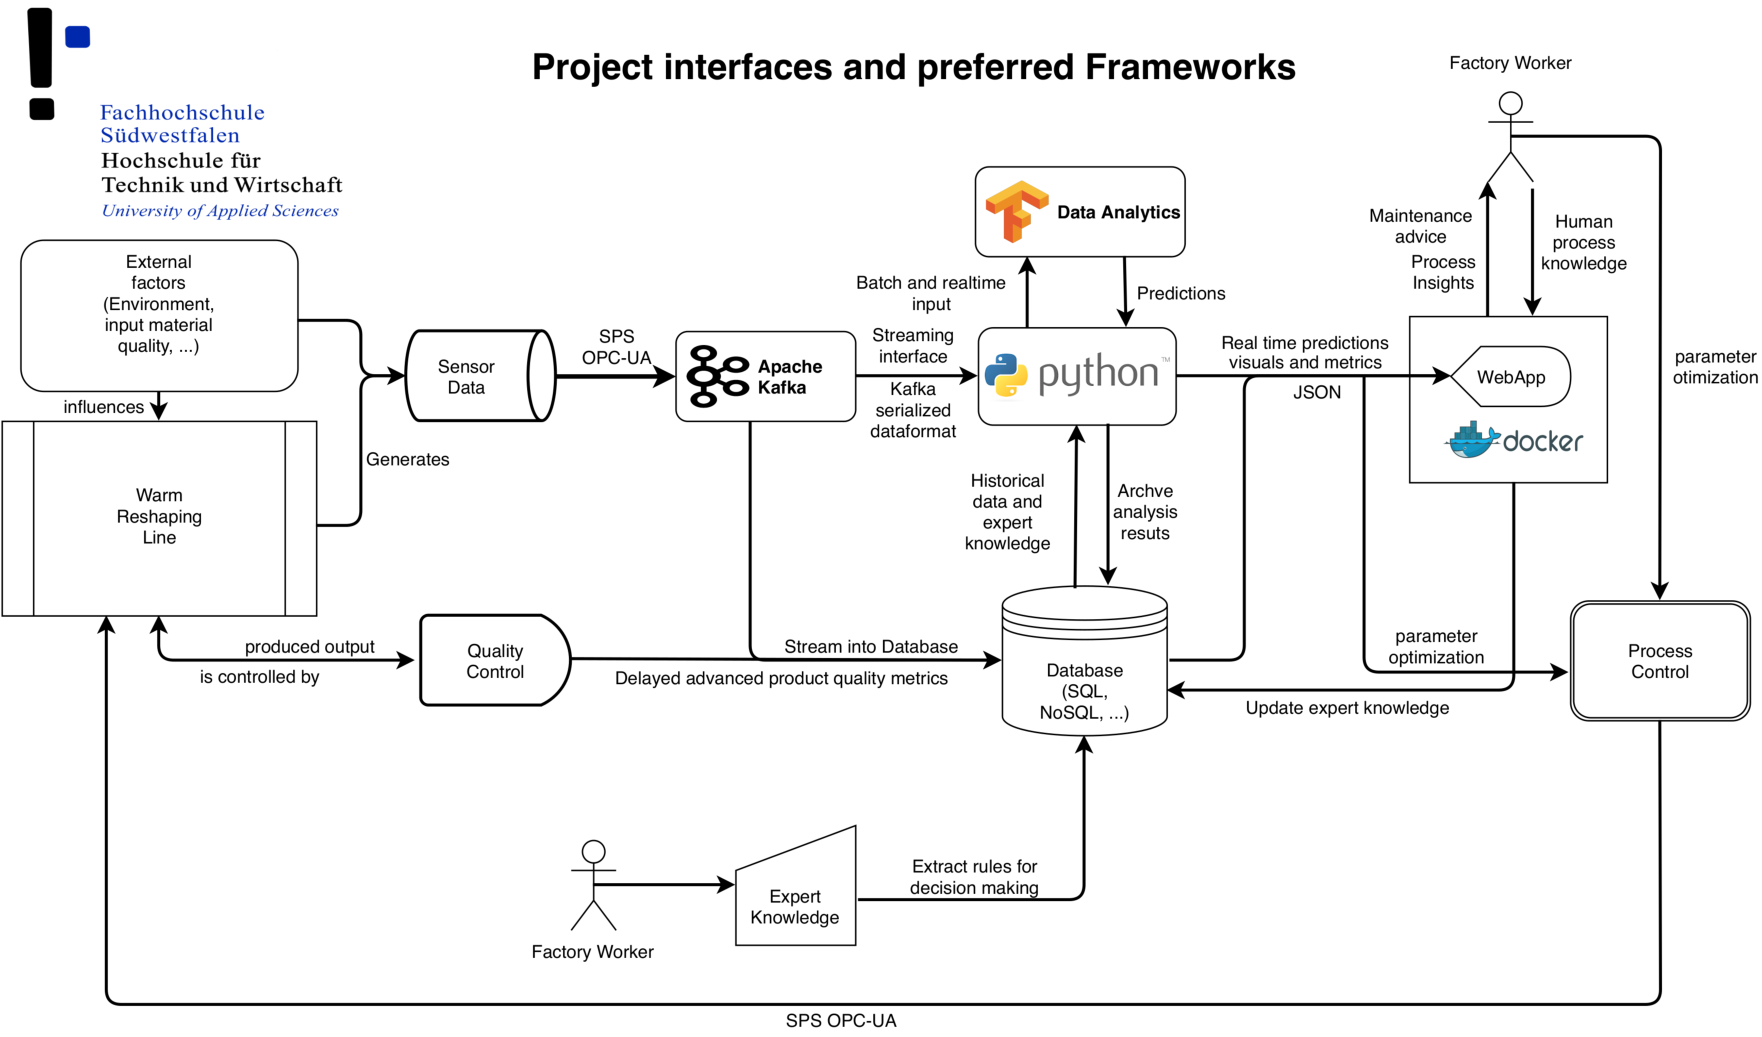
\includegraphics[width=0.4\textwidth]{images/process_v1_new.pdf}
                        %   \end{figure}
                        % \end{column}
                      \end{columns}
           \end{frame}

           \begin{frame}{Fallbeispiel: Vollautomatisierte Produktionszelle -- Darstellung der Daten für einen Maschinenoperator}
            \begin{columns}
              \begin{column}{0.6\textwidth}
                \begin{itemize}
                  \item Eine vereinfachte visuelle Darstellung der Maschinenparameter kann z.B. in einem Dashboard ausgegeben werden \newline
                  \item Erfahrene Operatoren können aus diesen Daten und ersten Analysen Schlussfolgerungen ziehen \newline
                  \item mögliche Parameteranpassungen im Prozess können durch diesen Operator durchgeführt werden
                \end{itemize}
              \end{column}
               % \begin{column}{0.4\textwidth}
               %   \begin{figure}
               %     \centering
               %      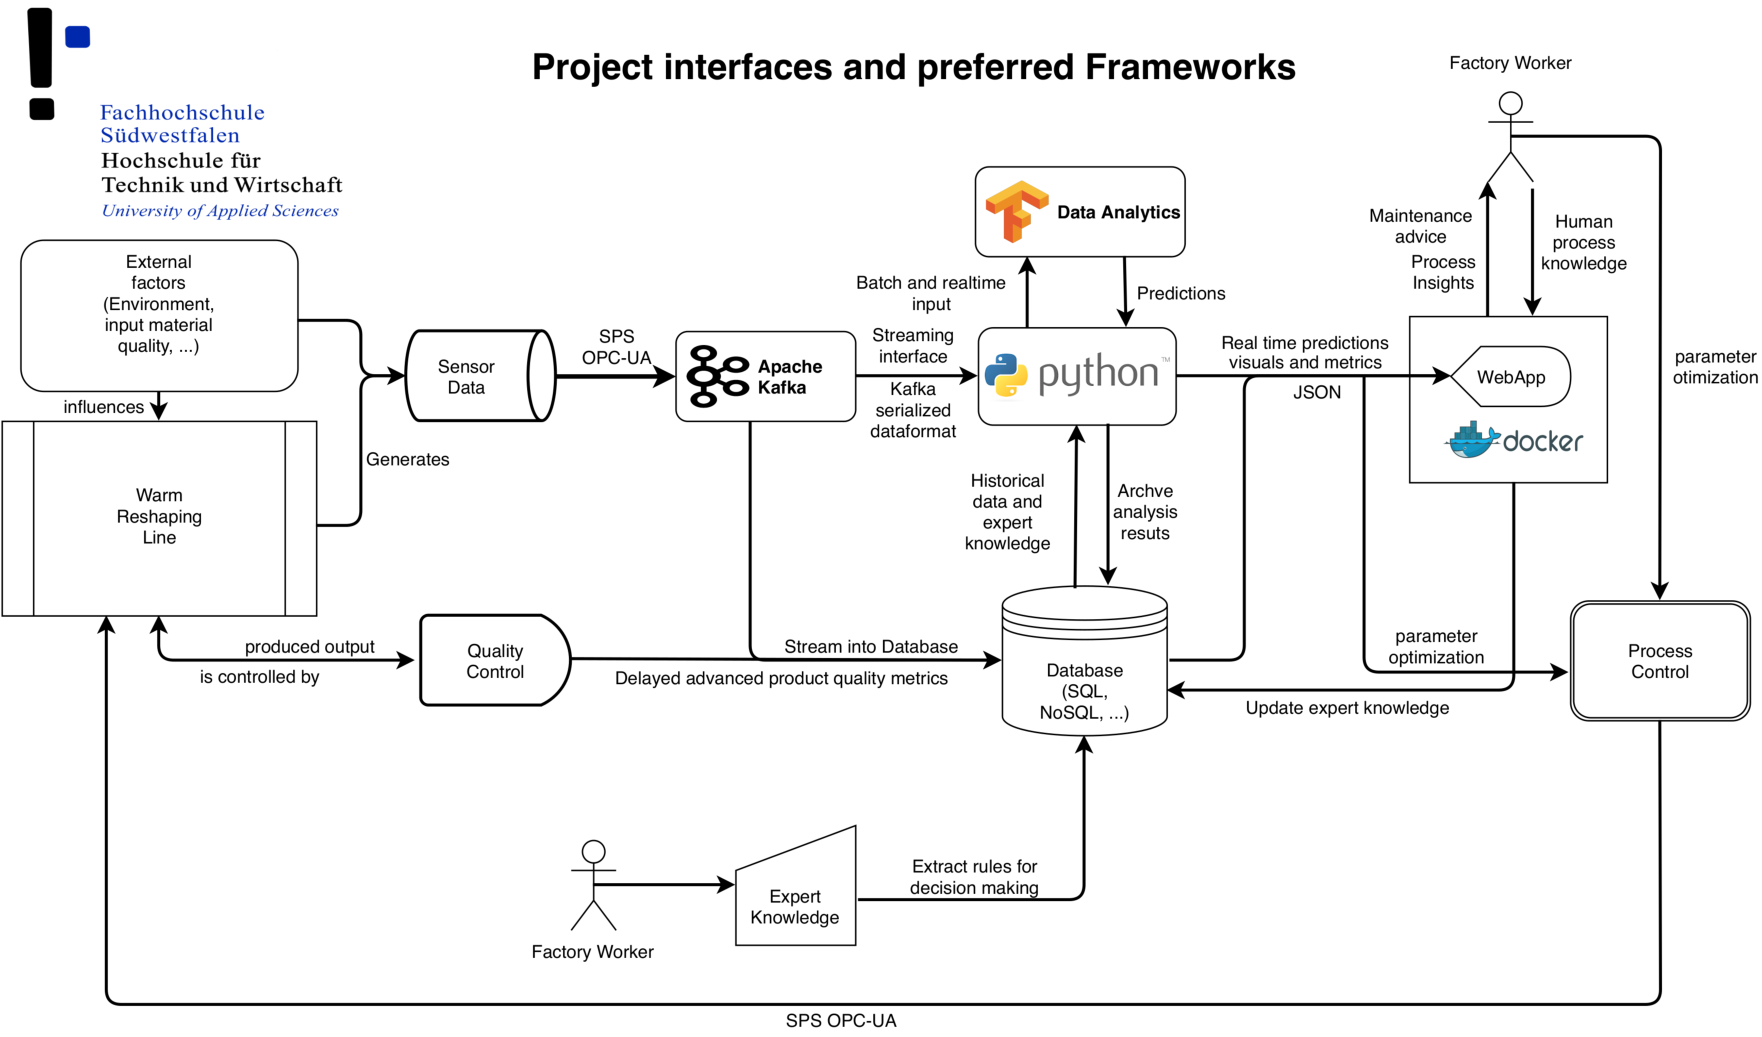
\includegraphics[width=0.4\textwidth]{images/process_v1_new.pdf}
               %   \end{figure}
              %  \end{column}
            \end{columns}
          \end{frame}

          \begin{frame}{Fallbeispiel: Vollautomatisierte Produktionszelle -- Direkte Handlungsanweisungen an einen Operator}
            \begin{columns}
              \begin{column}{0.6\textwidth}
                \begin{itemize}
                  \item Vorhersagen des trainierten Machine Learning Modells werden mit einer FMEA abgeglichen \newline
                  \item eine FMEA enthält die häufigsten Fehler und Defekte einer Analage \newline
                  \item Problemlösungen werden hier strukturiert skizziert \newline
                  \item unerfahrene Operatoren können hier durch das gesammelte Expertenwissen Entscheidungen treffen\newline
                  \item Operatoren können für den Vorhergesagten Zeitpunkt Mechaniker zur Wartung der Maschine anfordern
                \end{itemize}
              \end{column}
               % \begin{column}{0.4\textwidth}
               %   \begin{figure}
               %     \centering
               %      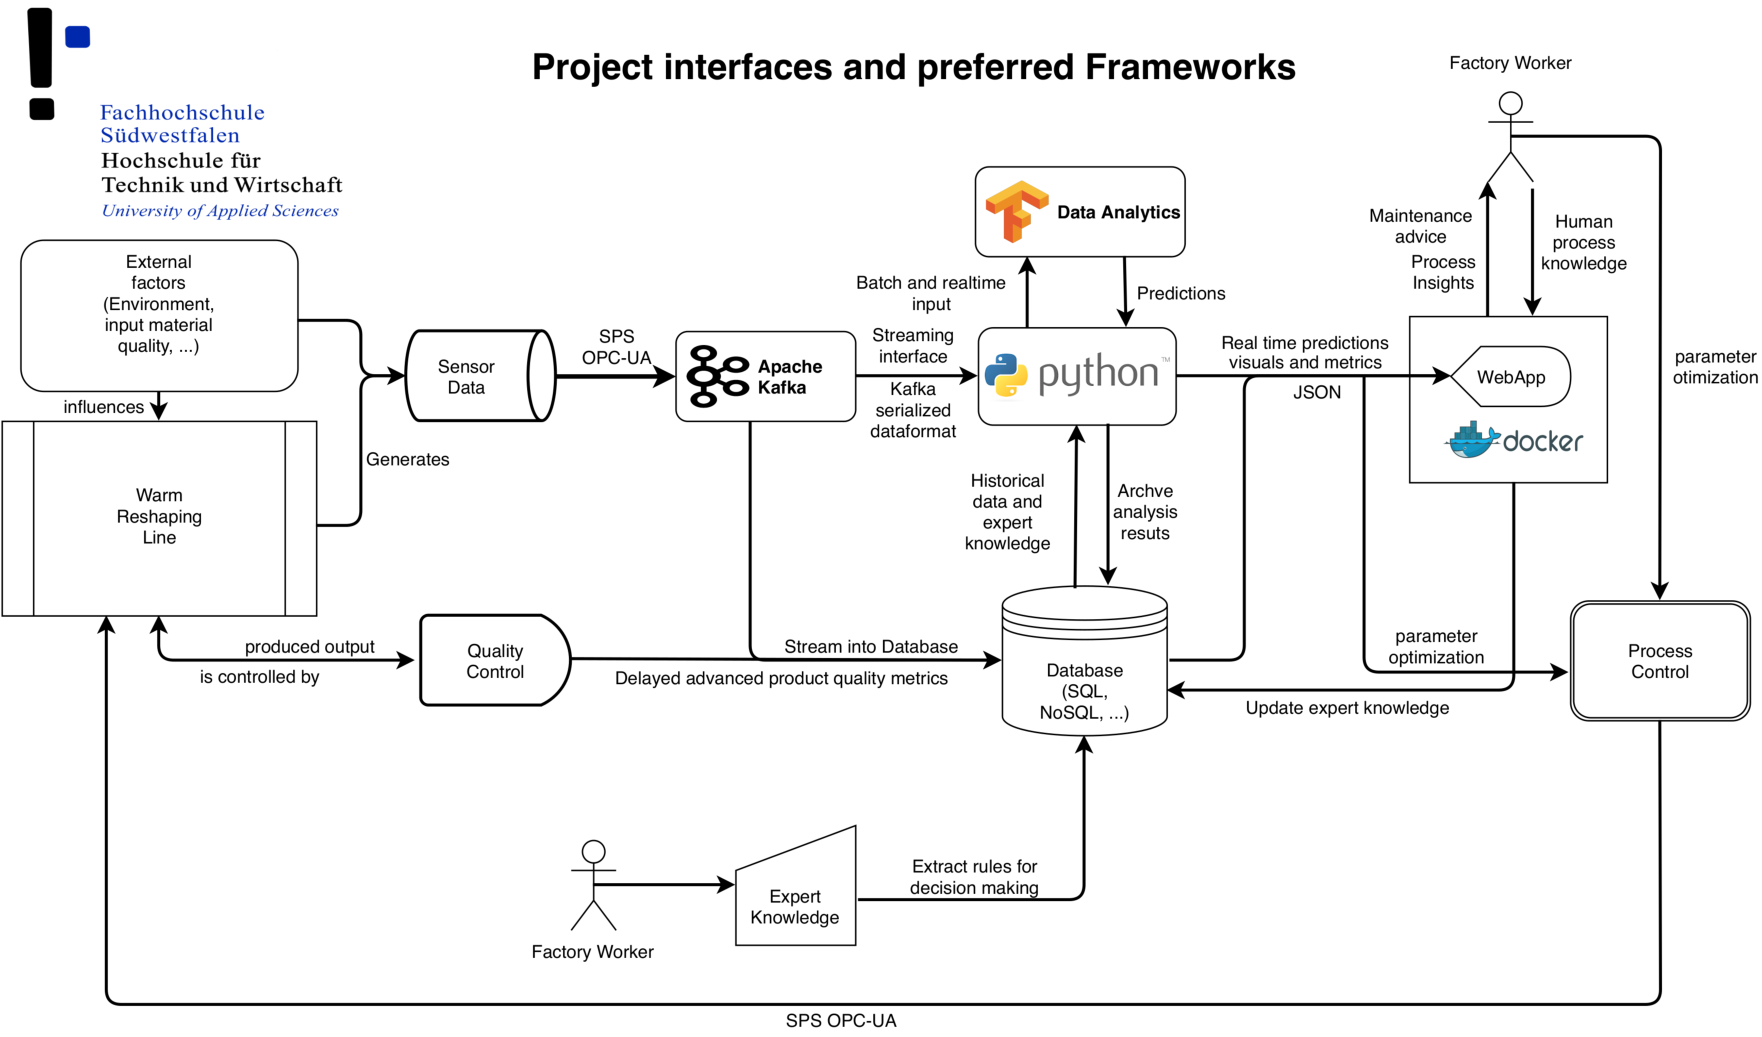
\includegraphics[width=0.4\textwidth]{images/process_v1_new.pdf}
               %   \end{figure}
              %  \end{column}
            \end{columns}
          \end{frame}


          \begin{frame}{Fallbeispiel: Vollautomatisierte Produktionszelle -- Direkte Handlungsanweisungen an die Prozessteuerung (Dangerzone)}
            \begin{columns}
              \begin{column}{0.6\textwidth}
                \begin{itemize}
                  \item Mögliche kritische Zustände können direkt zu einem Stop der Produktion führen \newline
                  \item Anpassung der Prozessparameter direkt durch die Software \rightarrow vollständig autonomes System \newline 
                  \item Mensch wird nur noch zum Eintragen von Know-How benötigt \newline
                \end{itemize}
              \end{column}
               % \begin{column}{0.4\textwidth}
               %   \begin{figure}
               %     \centering
               %      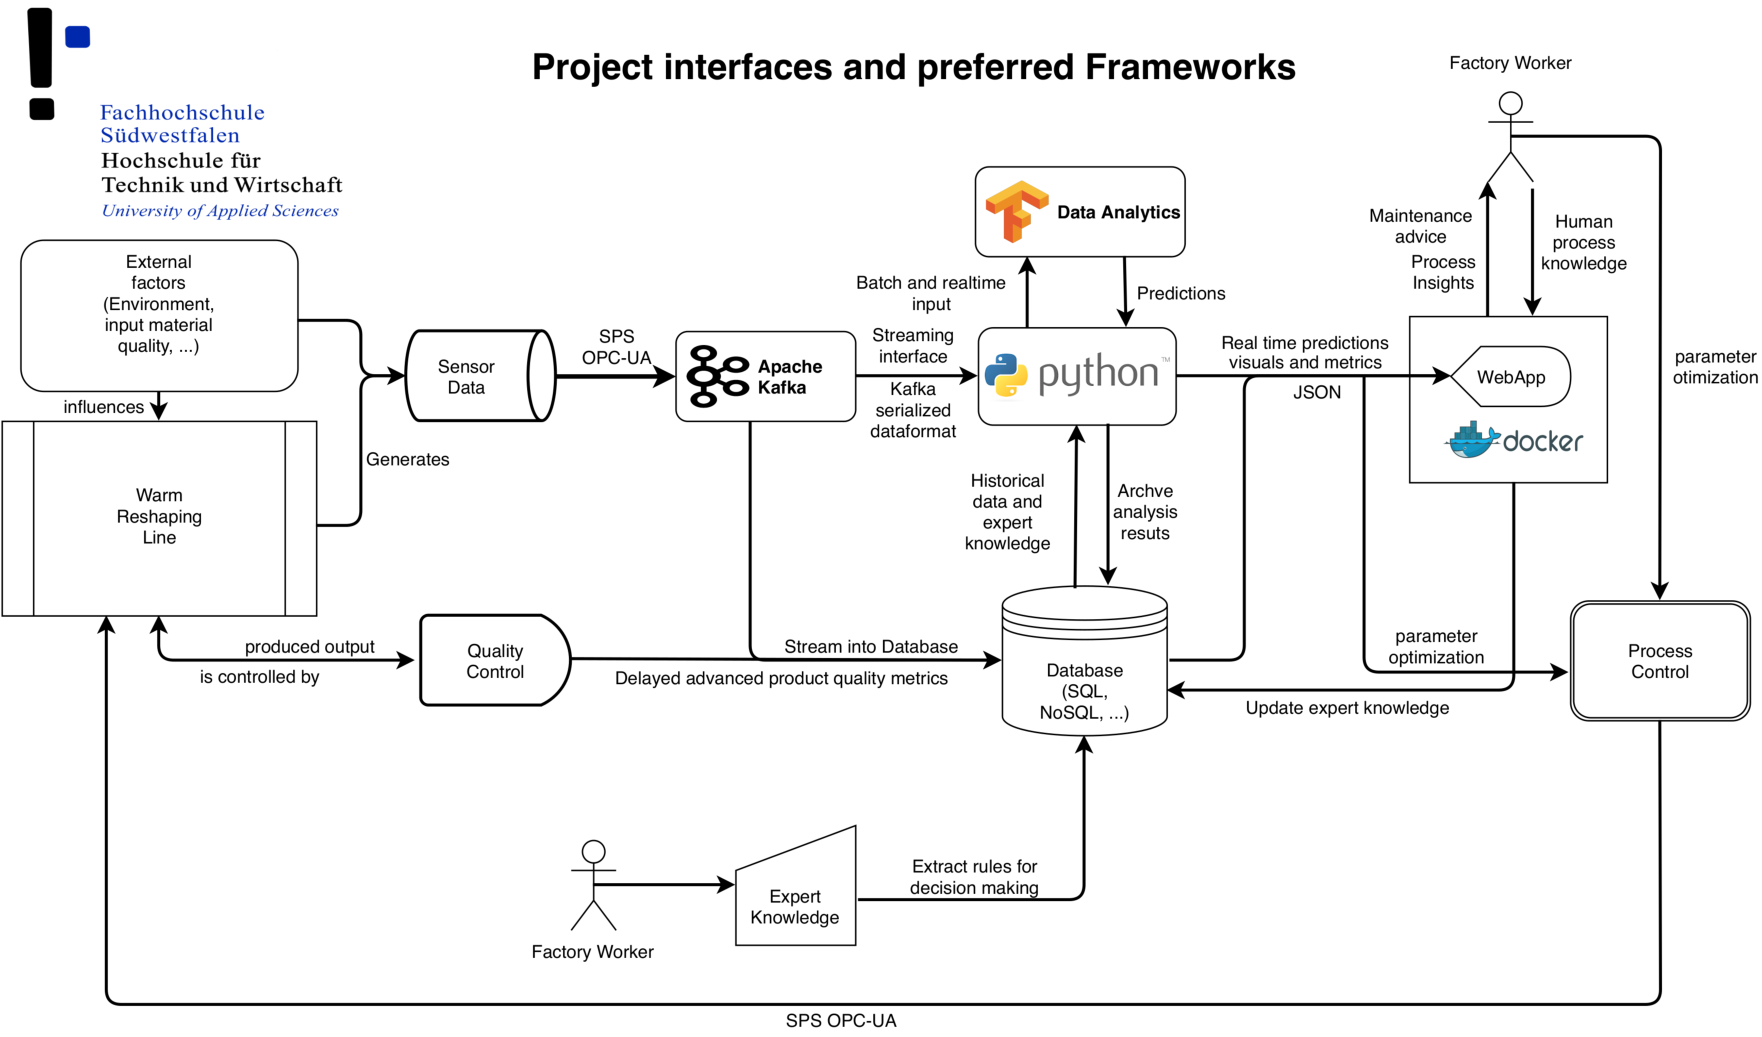
\includegraphics[width=0.4\textwidth]{images/process_v1_new.pdf}
               %   \end{figure}
              %  \end{column}
            \end{columns}
          \end{frame}

          
          \begin{frame}{Andere Beispiele: Wo ist PM finanziell besonders sinnvoll?}
            \begin{columns}
              \begin{column}{1\textwidth}
                \begin{itemize}
                  \item Kraftfahrzeuge: Sensorik in Verschleißteilen kann Totalausfälle vermeiden \newline
                  \item Luftfahrt: Der Ausfall von Passagier- oder Luftfrachtflügen kann mit guten Ausfallvorhersagen verhindert werden   \newline 
                  \item Schinenverkehr \newline
                \end{itemize}
              \end{column}
               % \begin{column}{0.4\textwidth}
               %   \begin{figure}
               %     \centering
               %      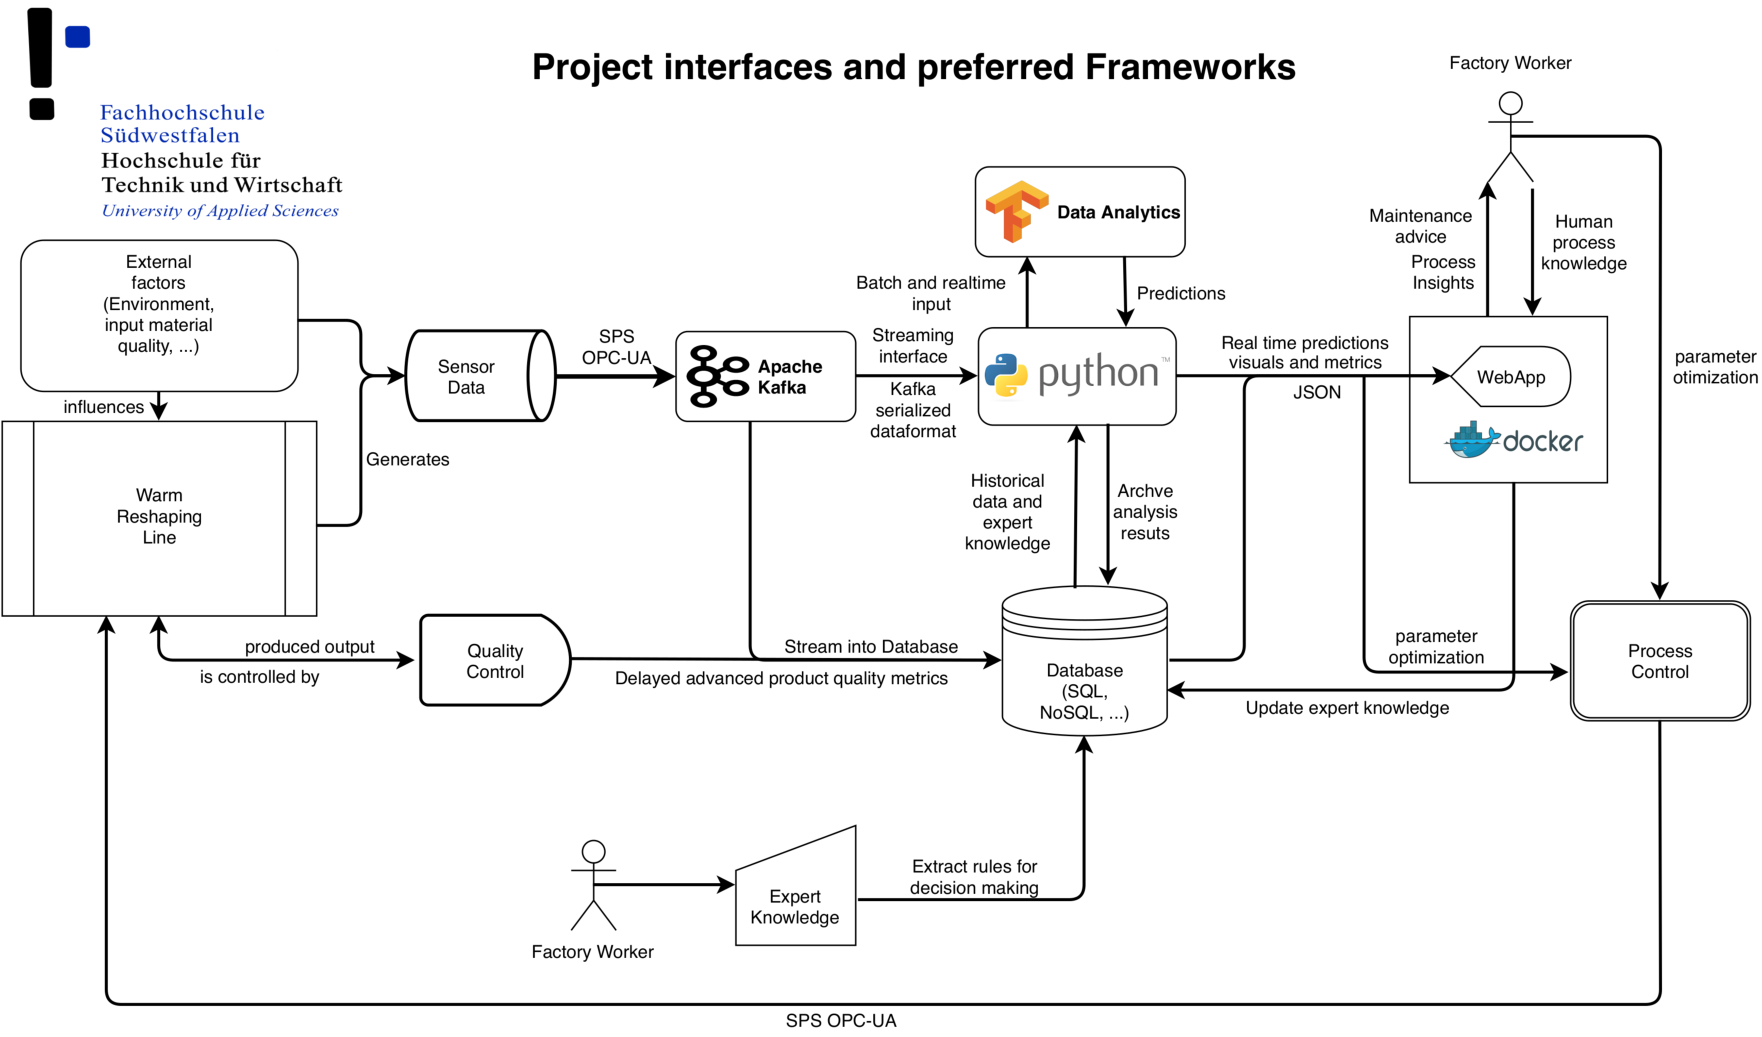
\includegraphics[width=0.4\textwidth]{images/process_v1_new.pdf}
               %   \end{figure}
               % \end{column}
            \end{columns}
          \end{frame}

% \begin{frame}{Experimental Setup -- What is the underlying process?}
%   \begin{columns}
%     \begin{column}{1\textwidth}
%     Process description
%       \begin{itemize}
%         \item Heating metal sheet to target temperature
%         \item Transfer to a hydraulic press
%         \item Reshaping the metal sheet while hot 
%         \item Cool down while in contact with cool surface using the correct cooling rate
%         \item Transfer to further manufacturing
%       \end{itemize}
%     \end{column}
%     \begin{column}{0\textwidth}
%    % \begin{figure}
%    % \centering
%    %             \includegraphics[width=0.9\textwidth]{images/intro/intro.pdf}
%    % \end{figure}
%     \end{column}
%   \end{columns}
% \end{frame}


% \begin{frame}{Experimental Setup -- What is the underlying process?}
%   \begin{center}
%    \smartdiagramset{border color=fhblue,
%    set color list={fhblue!35!white, fhblue!20!white, fhblue!20!white, fhblue!20!white, fhblue!20!white}}
%    \smartdiagram[sequence diagram]{Heating,
%    Transfer, Reshaping, Cooling, Manufacturing}
%   \end{center}
%   Heating metal sheet to target temperature
% \end{frame}
% 
% \begin{frame}[noframenumbering]{Experimental Setup -- What is the underlying process?}
%   \begin{center}
%     \smartdiagramset{border color=fhblue,set color list={fhblue!20!white, fhblue!35!white, fhblue!20!white, fhblue!20!white, fhblue!20!white}}
%     \smartdiagram[sequence diagram]{Heating,Transfer, Reshaping, Cooling, Manufacturing}
%   \end{center}
%   Transfer heated metal sheet into hydraulic press
% \end{frame}
% \begin{frame}[noframenumbering]{Experimental Setup -- What is the underlying process?}
%   \begin{center}
%   \smartdiagramset{border color=fhblue,set color list={fhblue!20!white, fhblue!20!white, fhblue!35!white, fhblue!20!white, fhblue!20!white}}
%   \smartdiagram[sequence diagram]{Heating,Transfer, Reshaping, Cooling, Manufacturing}
%   \end{center}
%    Reshaping of metal sheet while it's hot 
% \end{frame}
% 
% \begin{frame}[noframenumbering]{Experimental Setup -- What is the underlying process?}
%   \begin{center}
%     \smartdiagramset{border color=fhblue,  set color list={fhblue!20!white, fhblue!20!white, fhblue!20!white, fhblue!35!white, fhblue!20!white}}
%     \smartdiagram[sequence diagram]{Heating,  Transfer, Reshaping, Cooling, Manufacturing}
%   \end{center}
%   Cool down while in contact with coole surface with correct cooling rate 
% \end{frame}
% 
% \begin{frame}[noframenumbering]{Experimental Setup -- What is the underlying process?}
%   \begin{center}
%     \smartdiagramset{border color=fhblue, set color list={fhblue!20!white, fhblue!20!white, fhblue!20!white, fhblue!20!white, fhblue!35!white}}
%      \smartdiagram[sequence diagram]{Heating,     Transfer, Reshaping, Cooling, Manufacturing}
%   \end{center}
%   Transferring metal sheet to further manufacturing
% \end{frame}
%     
% % \begin{frame}{Development of the demonstration plant -- Why build one on our own?}
% % \begin{columns}
% %   \begin{column}{1\textwidth}
% %     \begin{itemize}
% % 
% %       \item Sensors
% %       \begin{itemize}
% %         \item[\rightarrow] Possible sensors for later implementation in production plants
% %         \item[\rightarrow] Temperature monitoring with infrared cameras
% %         \item[\rightarrow] Temperature Sensors in the stamp
% %       \end{itemize}
%       \item Implementation of a completely automonous system 
%       \begin{itemize}
%         \item[\rightarrow] Edge computing on site
%         \item[\rightarrow] Backend development\newline
%       \end{itemize}
%       
%       %mit bildern/video
%     \end{itemize}
%   \end{column}
%   \begin{column}{0.6\textwidth}
%  % \begin{figure}
%  %  \centering
%  %  \includegraphics[width=0.9\textwidth]{images/intro/intro.pdf}
%  % \end{figure}
%   \end{column}
% \end{columns}
% \end{frame}




\begin{frame}[allowframebreaks]{References}
 \bibliographystyle{ieeetr}
 \bibliography{lit.bib}
\end{frame}
\end{document}
